%=======================02-713 LaTeX template, following the 15-210 template==================
%
% You don't need to use LaTeX or this template, but you must turn your homework in as
% a typeset PDF somehow.
%
% How to use:
%    1. Update your information in section "A" below
%    2. Write your answers in section "B" below. Precede answers for all 
%       parts of a question with the command "\question{n}{desc}" where n is
%       the question number and "desc" is a short, one-line description of 
%       the problem. There is no need to restate the problem.
%    3. If a question has multiple parts, precede the answer to part x with the
%       command "\part{x}".
%    4. If a problem asks you to design an algorithm, use the commands
%       \algorithm, \correctness, \runtime to precede your discussion of the 
%       description of the algorithm, its correctness, and its running time, respectively.
%    5. You can include graphics by using the command \includegraphics{FILENAME}
%
\documentclass[11pt]{article}
\usepackage{amsmath,amssymb,amsthm}
\usepackage{graphicx}
\usepackage[margin=1in]{geometry}
\usepackage{fancyhdr}
\usepackage{listings}
\usepackage{float} 
\usepackage{subfig}

\setlength{\parindent}{0pt}
\setlength{\parskip}{5pt plus 1pt}
\setlength{\headheight}{13.6pt}
\newcommand\question[2]{\vspace{.25in}\hrule\textbf{#1: #2}\vspace{.5em}\hrule\vspace{.10in}}
\renewcommand\part[1]{\vspace{.10in}\textbf{(#1)}}
\newcommand\one{\vspace{.10in}\textbf{Step1: }}
\newcommand\two{\vspace{.10in}\textbf{Step2: }}
\newcommand\three{\vspace{.10in}\textbf{Step3: }}
\newcommand\four{\vspace{.10in}\textbf{Step4: }}
\pagestyle{fancyplain}
\lhead{\textbf{\NAME\ (\ANDREWID)}}
\chead{\textbf{ASS\HWNUM}}
\rhead{\today}
\begin{document}\raggedright
%Section A==============Change the values below to match your information==================
\newcommand\NAME{Yao Xiao}  % your name
\newcommand\ANDREWID{2019180015}     % your andrew id
\newcommand\HWNUM{2}              % the homework number
%Section B==============Put your answers to the questions below here=======================

% no need to restate the problem --- the graders know which problem is which,
% but replacing "The First Problem" with a short phrase will help you remember
% which problem this is when you read over your homeworks to study.
\question{1}{The First Problem}
\part{a} \one Randomly prepare the training and test data.\\

\begin{lstlisting}
    unsigned seed = std::chrono::system_clock::now().time_since_epoch().count();
    std::shuffle(tmp.begin(), tmp.end(), std::default_random_engine(seed));

    int testNum = int(tmp.size() / (1 + ratio));
    cout << "Test Number: " << testNum << endl;
    cout << "Total Number: " << tmp.size() << endl;
    int trainNum = tmp.size() - testNum;
    cout << "Train Number: " << trainNum << endl;
    ofstream outfile;
    outfile.open("../test.txt", ios::app);
    for (int i = 0; i < testNum; i++) {
        outfile << tmp[i] << endl;
    }

    ofstream output;
    output.open("../train.txt", ios::app);
    for (int i = testNum; i < tmp.size(); i++) {
        output << tmp[i] << endl;
    }
    output.close();
\end{lstlisting}

\begin{figure}[H]
    \centering
    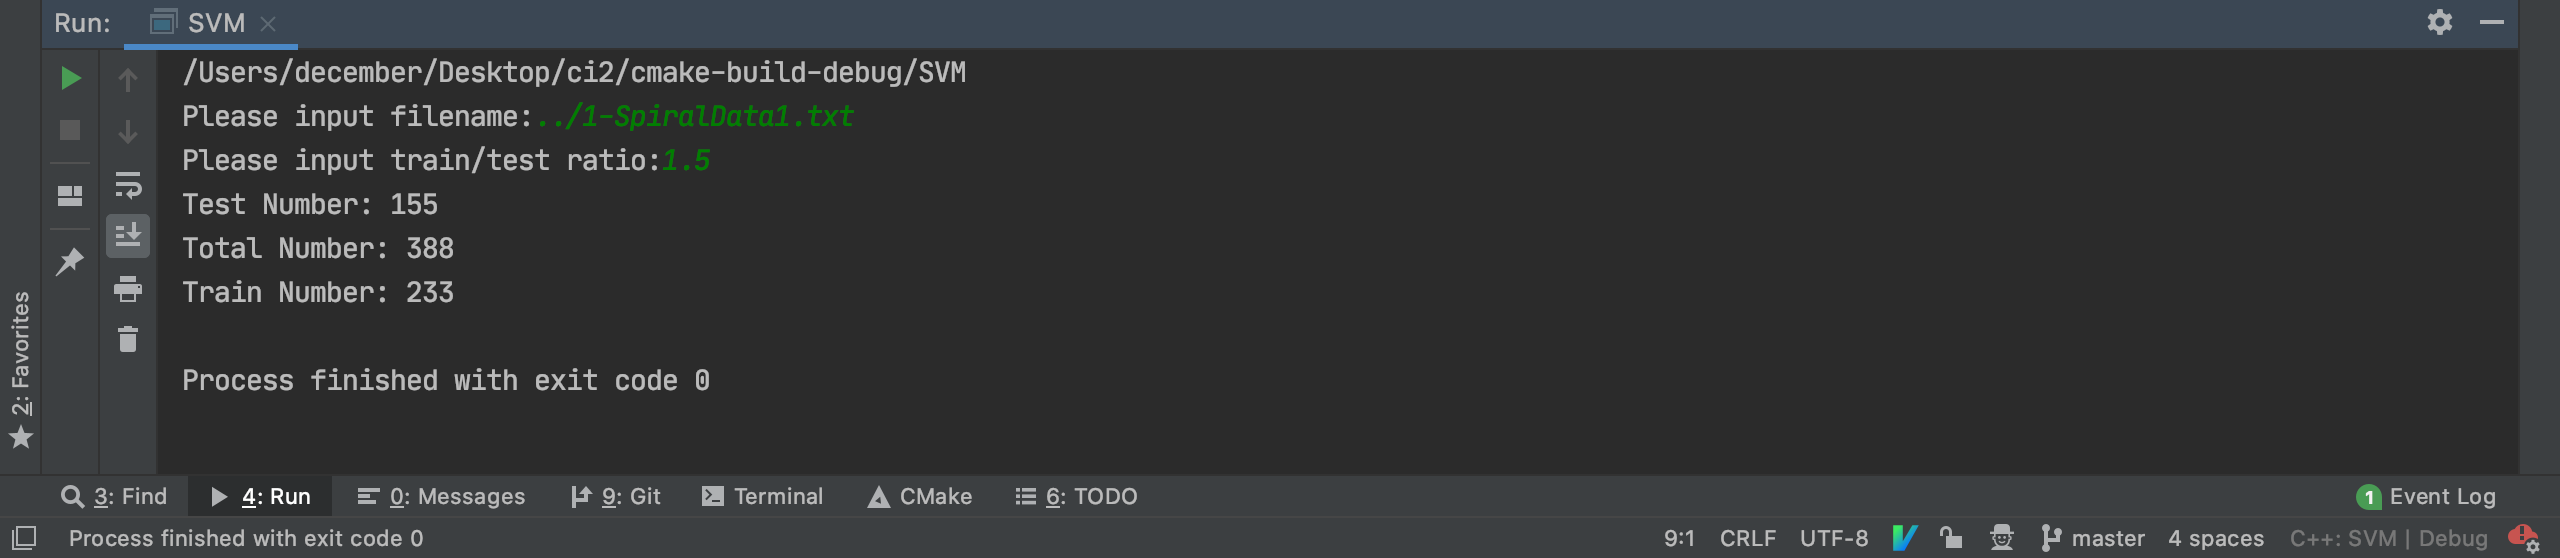
\includegraphics[width=0.8\textwidth]{gd1}
    \caption{Data1}
\end{figure}

\begin{figure}[H]
    \centering
    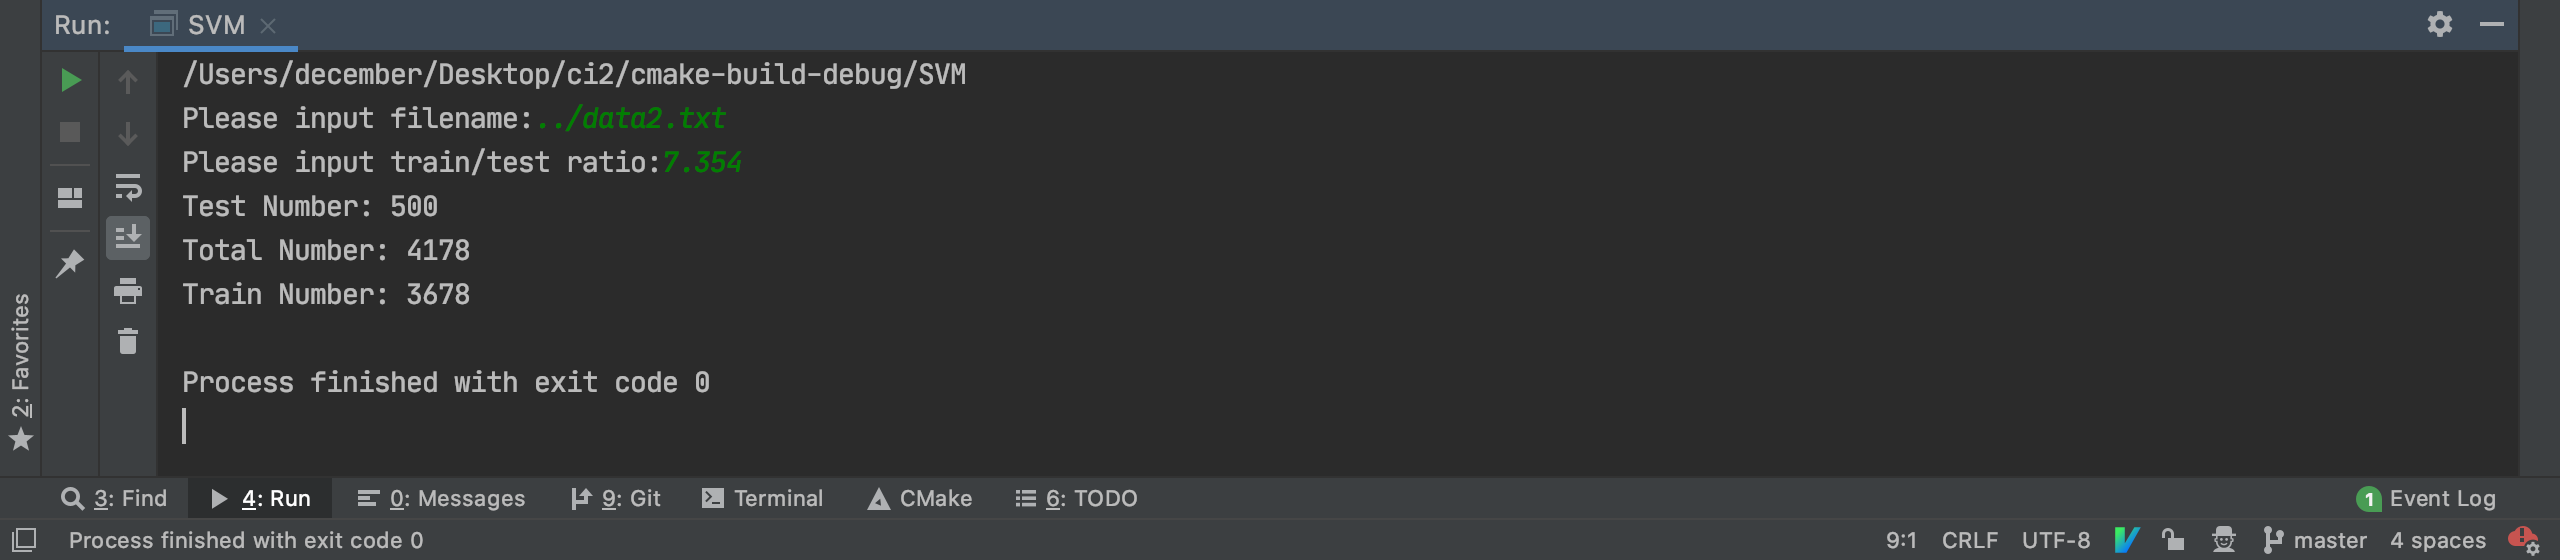
\includegraphics[width=0.8\textwidth]{gd2}
    \caption{Data2}
\end{figure}

\begin{figure}[H]
    \centering
    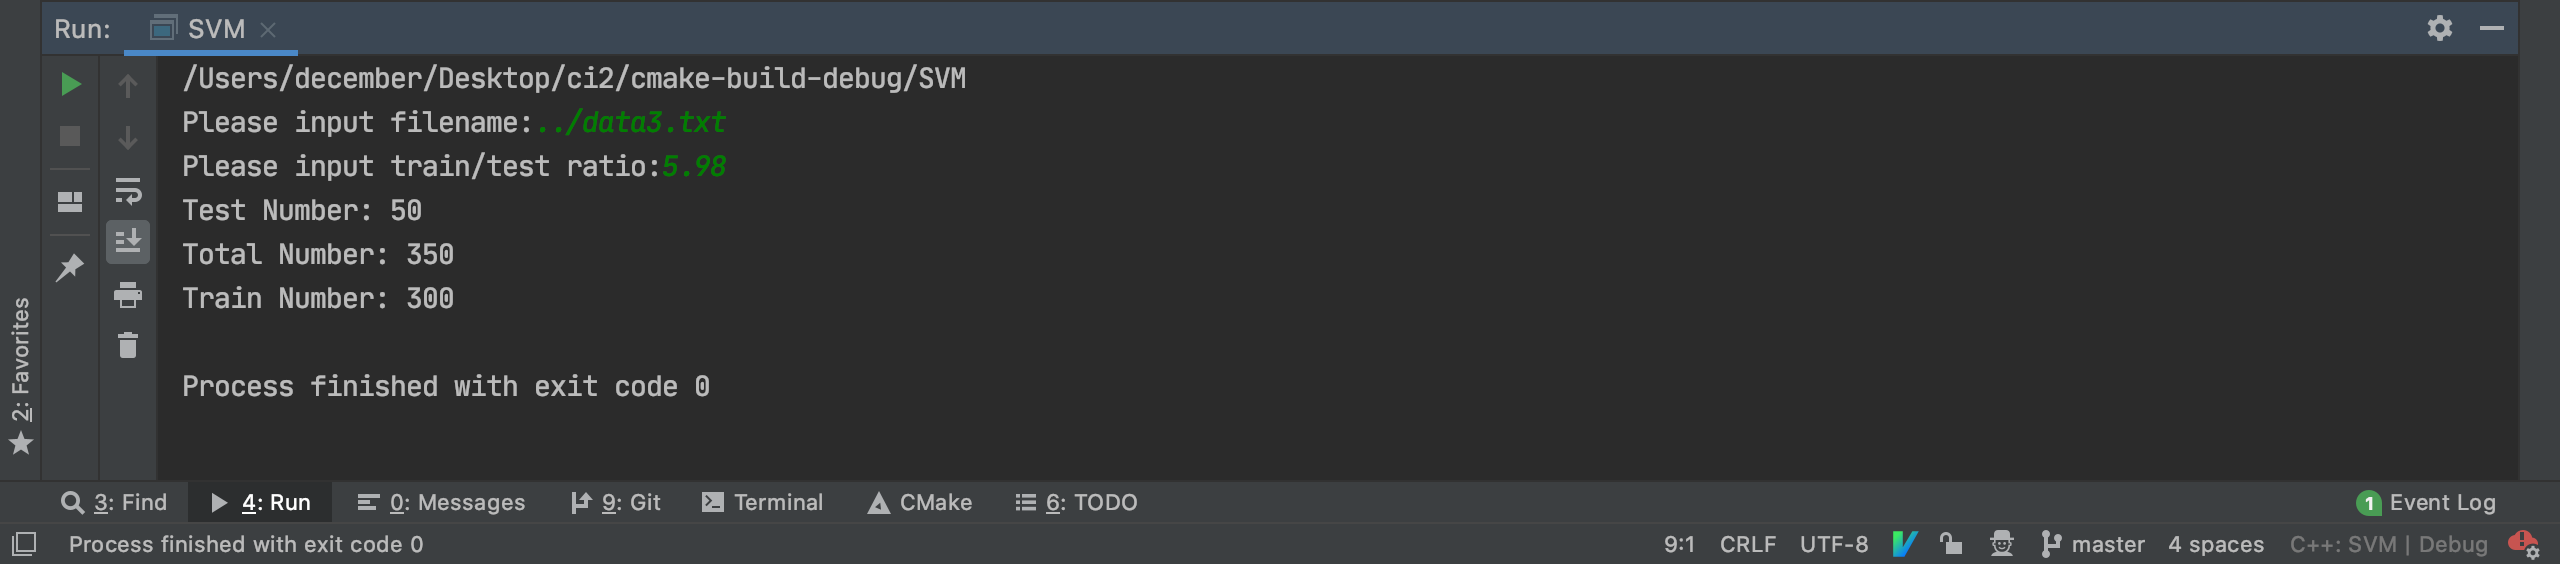
\includegraphics[width=0.8\textwidth]{gd3}
    \caption{Data3}
\end{figure}

\part{b} \two Adjust SVM parameters and test the best accuracy. \\

\begin{figure}[H]
    \centering
    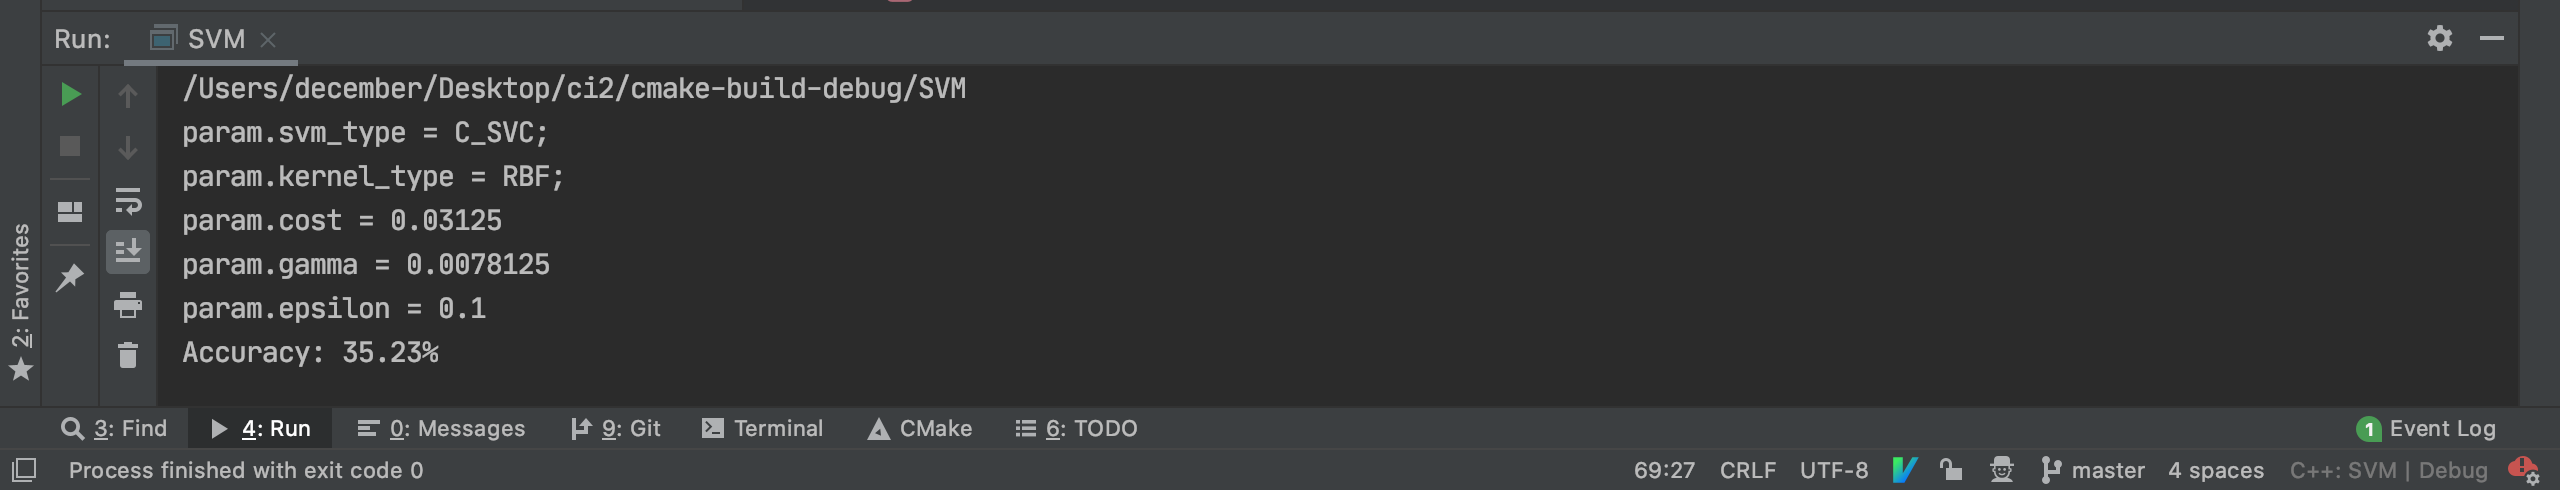
\includegraphics[width=0.8\textwidth]{d1p1}
    \caption{Adjust parameters on data1}
\end{figure}

For dataset 2, the effect of optimization is still not ideal.\\

\begin{figure}[H]
    \centering
    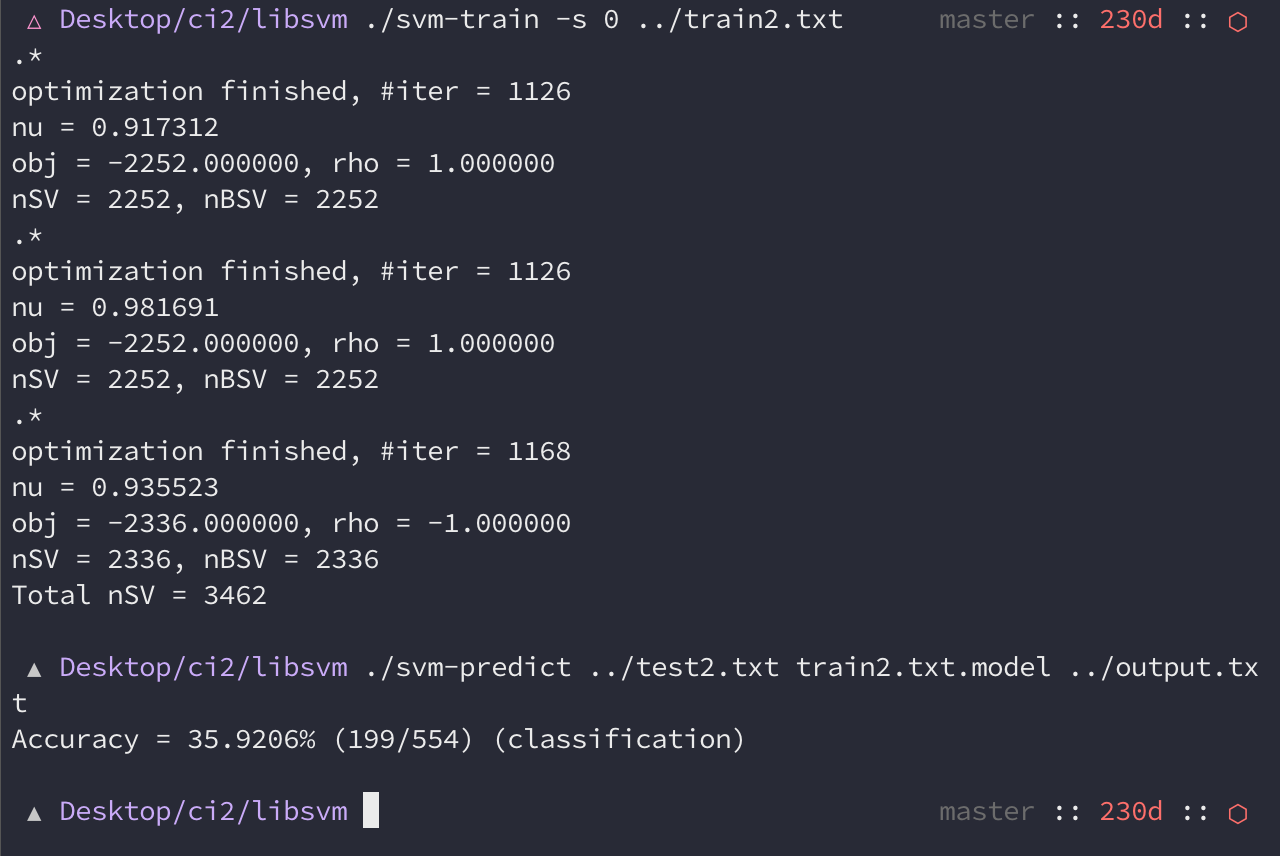
\includegraphics[width=0.6\textwidth]{d2p1}
    \caption{Adjust parameters on data2}
\end{figure}

\begin{figure}[H]
    \centering
    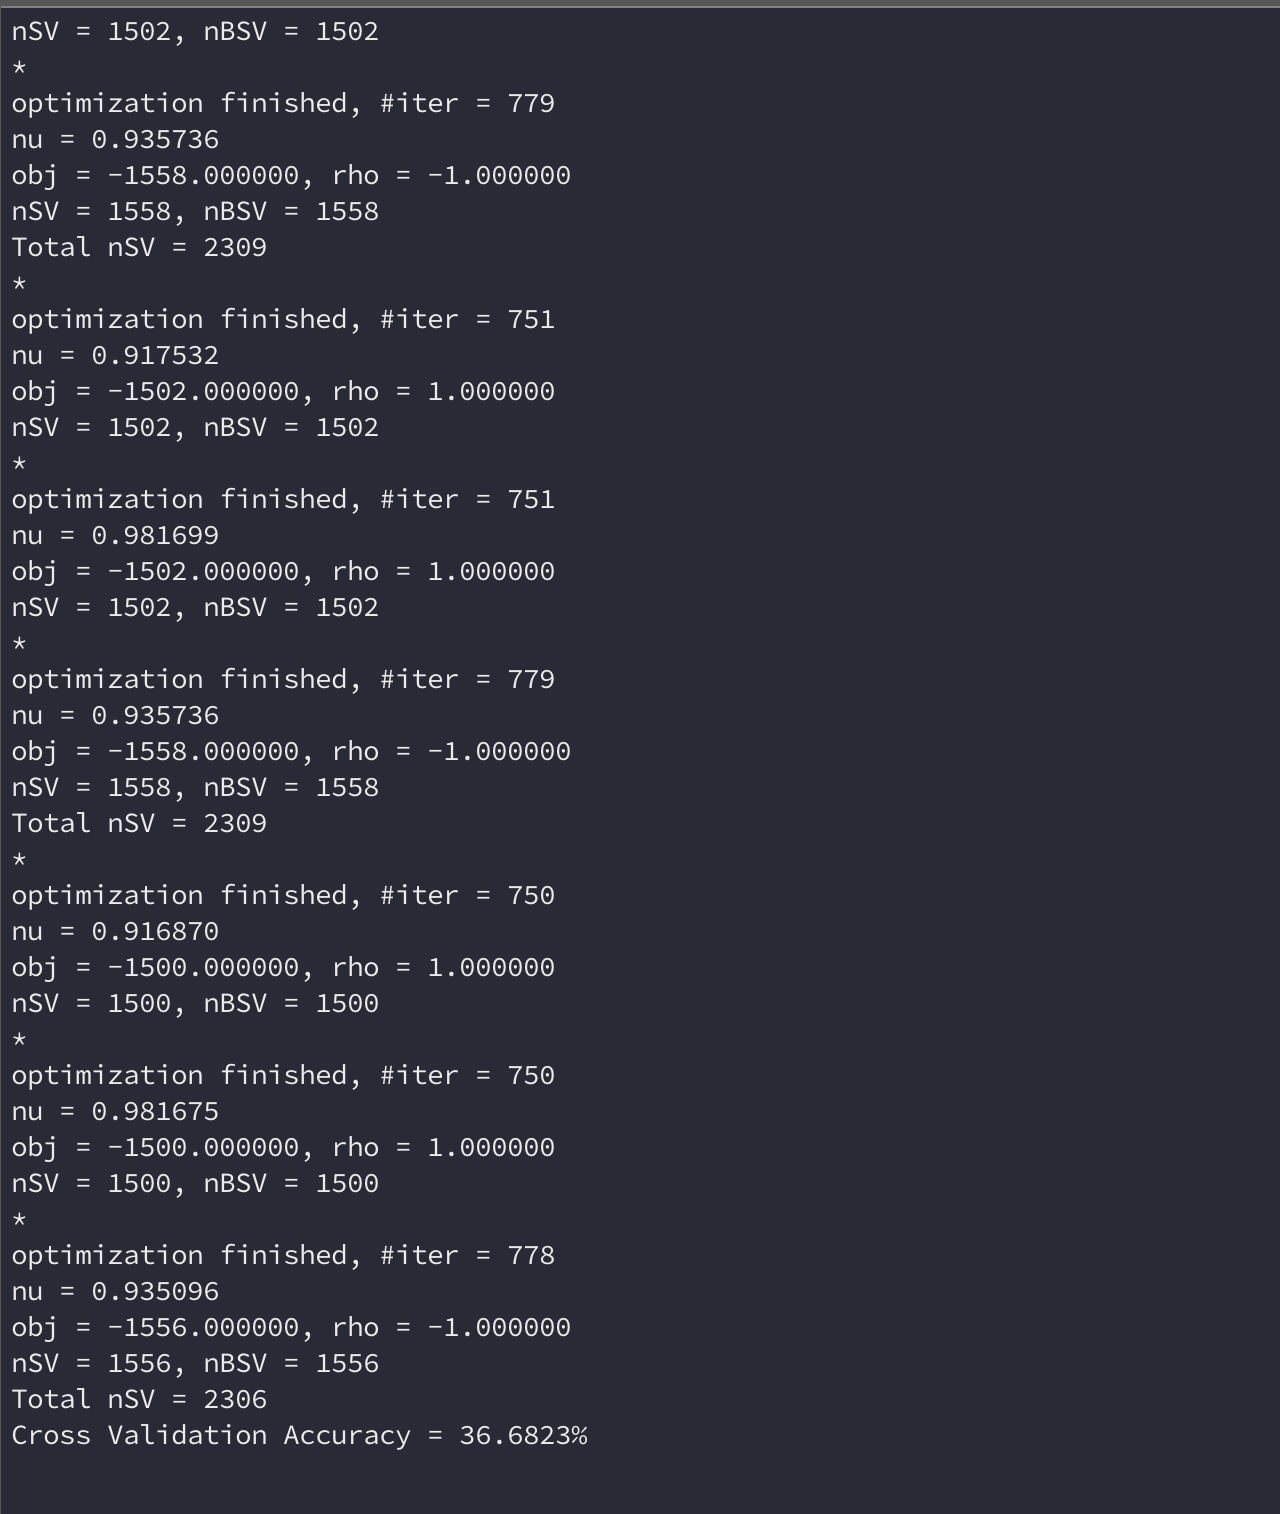
\includegraphics[width=0.6\textwidth]{d2p2}
    \caption{Adjust parameters on data2}
\end{figure}

\begin{figure}[H]
    \centering
    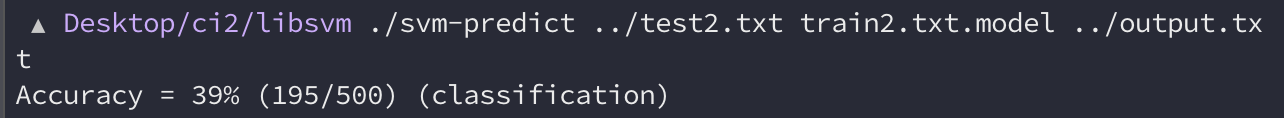
\includegraphics[width=0.6\textwidth]{d2p2-2}
    \caption{Adjust parameters on data2}
\end{figure}

When optimizing dataset 3, it is found that there is no obvious difference between the linear and rbf kernels, but the linear speed is faster.\\

\begin{figure}[H]
    \centering
    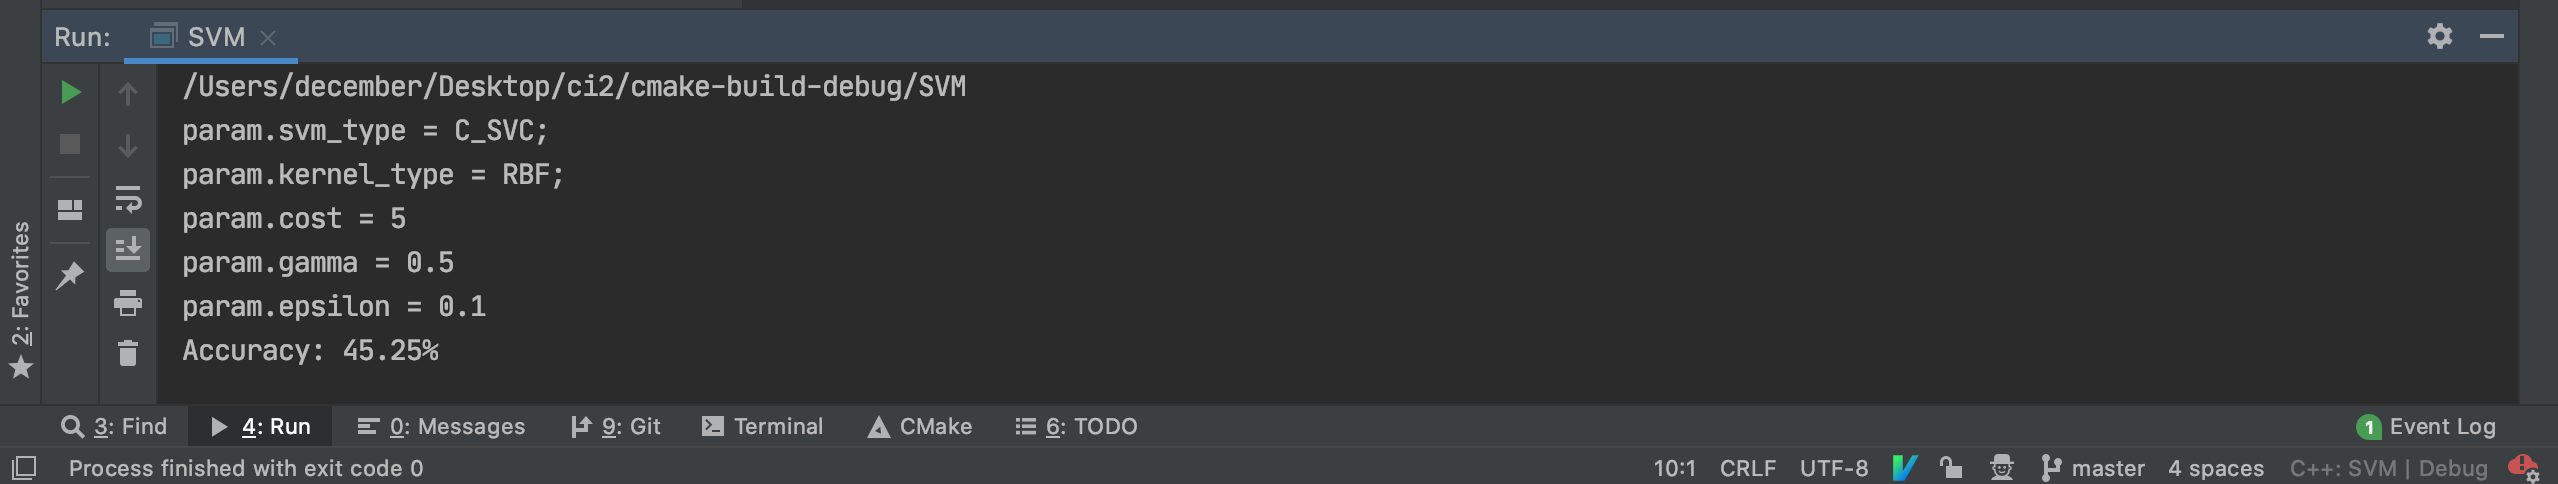
\includegraphics[width=0.8\textwidth]{d3p1}
    \caption{Adjust parameters on data3}
\end{figure}

\begin{figure}[H]
    \centering
    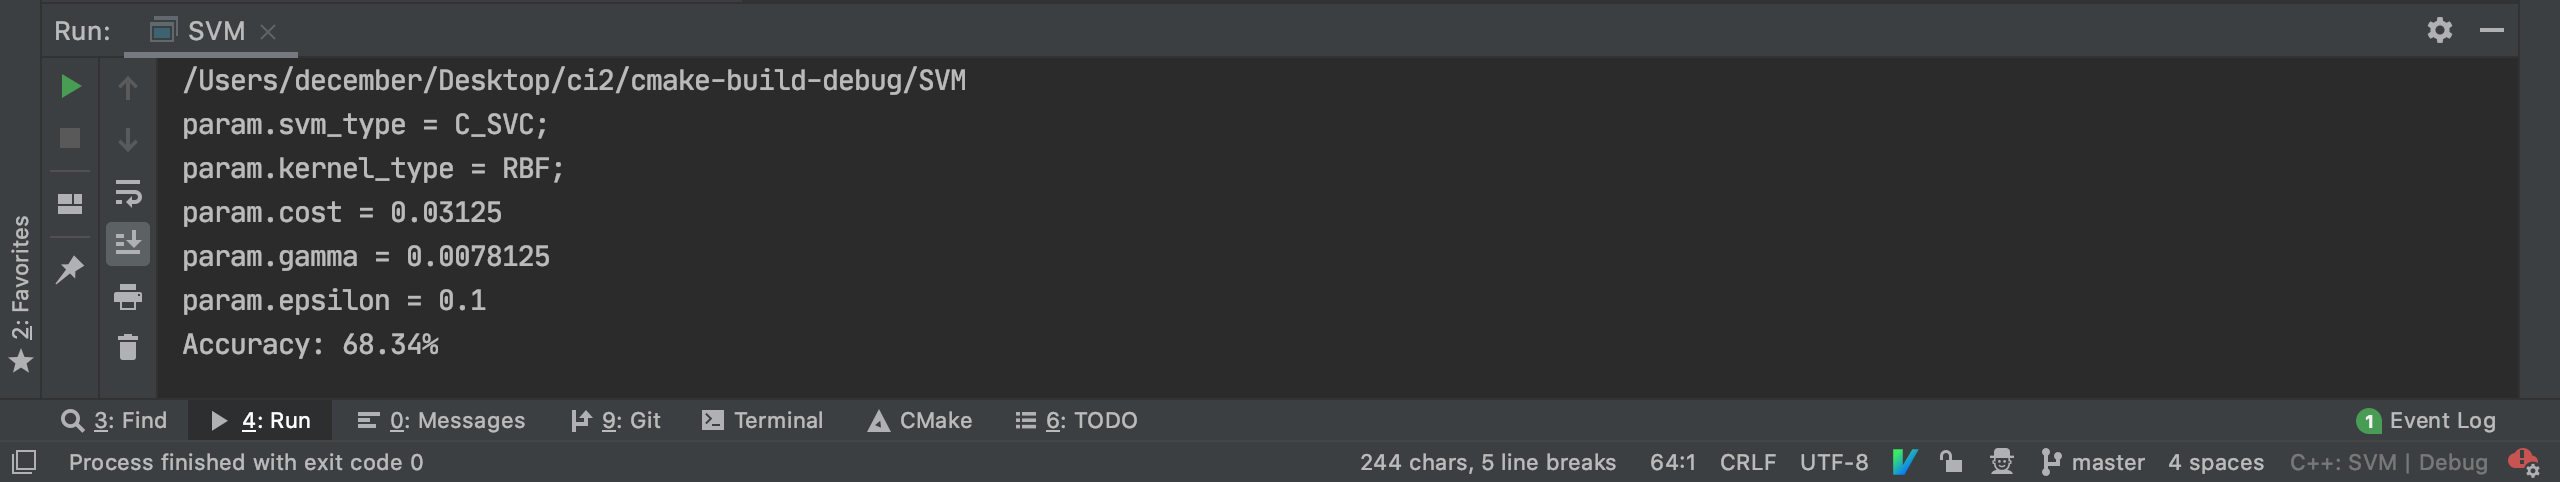
\includegraphics[width=0.8\textwidth]{d3p2}
    \caption{Adjust parameters on data3}
\end{figure}

\begin{figure}[H]
    \centering
    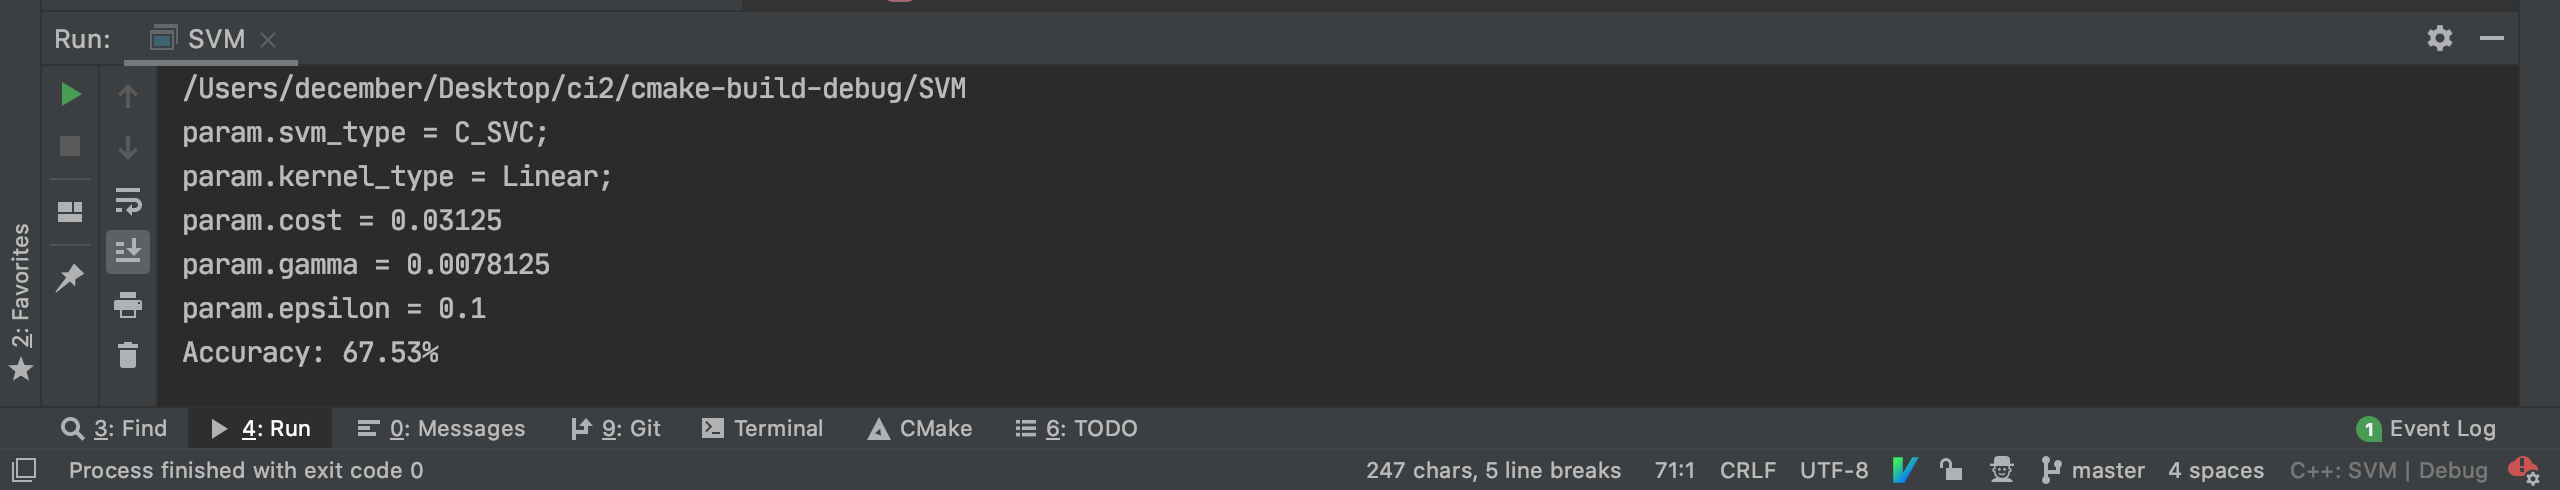
\includegraphics[width=0.8\textwidth]{d3p3}
    \caption{Adjust parameters on data3}
\end{figure}




\question{2}{The Second Problem} 

\part{a} \one Implement four functions
\begin{lstlisting}
void InitPop(int ***CrntPop, int ***NextPop, int **Fitness, int **BestMember, double **rFitness) {
    int i, j, t, temp;
    srand(Seed);
    *CrntPop = new int *[cPopSize];
    *NextPop = new int *[cPopSize];
    for (i = 0; i < cPopSize; i++) {
        (*CrntPop)[i] = new int[cIndividualLength];
        (*NextPop)[i] = new int[cIndividualLength];
    }
    *Fitness = new int[cPopSize];
    *rFitness = new double[cPopSize];
    *BestMember = new int[cIndividualLength];
    if (Fitness == NULL || BestMember == NULL)exit(1);
    for (i = 0; i < cPopSize; i++) {
        for (j = 0; j < cIndividualLength; j++)
            (*CrntPop)[i][j] = j;
        for (j = 0; j < cIndividualLength; j++) {
            temp = RandInt(cIndividualLength);
            t = (*CrntPop)[i][j];
            (*CrntPop)[i][j] = (*CrntPop)[i][temp];
            (*CrntPop)[i][temp] = t;
        }
    }
}

int EvaluateFitness(int *Member) {
    //Evaluate the fitness function from distance table
    int p1, p2;
    int TheFitness = 0;
    for (int i = 1; i < cIndividualLength; i++) {
        p1 = Member[i];
        p2 = Member[i - 1];
        TheFitness += lookupTable[p1][p2];
    }
    return (TheFitness);
}

void Crossover(int *P1, int *P2, int *C1, int *C2) {
    int i, Left, Right;
    switch (CrossoverType) {
        case eRandom: // swap random genes
            for (i = 0; i < cIndividualLength; i++) {





\question{2}{The Second Problem} 

\part{a} \one Implement four functions
\begin{lstlisting}
void InitPop(int ***CrntPop, int ***NextPop, int **Fitness, int **BestMember, double **rFitness) {
    int i, j, t, temp;
    srand(Seed);
    *CrntPop = new int *[cPopSize];
    *NextPop = new int *[cPopSize];
    for (i = 0; i < cPopSize; i++) {
        (*CrntPop)[i] = new int[cIndividualLength];
        (*NextPop)[i] = new int[cIndividualLength];
    }
    *Fitness = new int[cPopSize];
    *rFitness = new double[cPopSize];
    *BestMember = new int[cIndividualLength];
    if (Fitness == NULL || BestMember == NULL)exit(1);
    for (i = 0; i < cPopSize; i++) {
        for (j = 0; j < cIndividualLength; j++)
            (*CrntPop)[i][j] = j;
        for (j = 0; j < cIndividualLength; j++) {
            temp = RandInt(cIndividualLength);
            t = (*CrntPop)[i][j];
            (*CrntPop)[i][j] = (*CrntPop)[i][temp];
            (*CrntPop)[i][temp] = t;
        }
    }
}

int EvaluateFitness(int *Member) {
    //Evaluate the fitness function from distance table
    int p1, p2;
    int TheFitness = 0;
    for (int i = 1; i < cIndividualLength; i++) {
        p1 = Member[i];
        p2 = Member[i - 1];
        TheFitness += lookupTable[p1][p2];
    }
    return (TheFitness);
}

void Crossover(int *P1, int *P2, int *C1, int *C2) {
    int i, Left, Right;
    switch (CrossoverType) {
        case eRandom: // swap random genes
            for (i = 0; i < cIndividualLength; i++) {
                if (RandInt(2)) {
                    C1[i] = P1[i];
                    C2[i] = P2[i];
                } else {
                    C1[i] = P2[i];
                    C2[i] = P1[i];
                }
            }
            break;
        case eUniform: // swap odd/even genes
            for (i = 0; i < cIndividualLength; i++) {
                if (i % 2) {
                    C1[i] = P1[i];
                    C2[i] = P2[i];
                } else {
                    C1[i] = P2[i];
                    C2[i] = P1[i];
                }
            }
            break;
        case eOnePoint:  // perform 1 point x-over
            Left = RandInt(cIndividualLength);
            if (cDebug) {
                printf("Cut points: 0 <= %d <= %d\n", Left, cIndividualLength - 1);
            }
            for (i = 0; i <= Left; i++) {
                C1[i] = P1[i];
                C2[i] = P2[i];
            }
            for (i = Left + 1; i < cIndividualLength; i++) {
                C1[i] = P2[i];
                C2[i] = P1[i];
            }
            break;
        case eTwoPoint:  // perform 2 point x-over
            Left = RandInt(cIndividualLength - 1);
            Right = Left + 1 + RandInt(cIndividualLength - Left - 1);
            if (cDebug) {
                printf("Cut points: 0 <= %d < %d <= %d\n", Left, Right, cIndividualLength - 1);
            }
            for (i = 0; i <= Left; i++) {
                C1[i] = P1[i];
                C2[i] = P2[i];
            }
            for (i = Left + 1; i <= Right; i++) {
                C1[i] = P2[i];
                C2[i] = P1[i];
            }
            for (i = Right + 1; i < cIndividualLength; i++) {
                C1[i] = P1[i];
                C2[i] = P2[i];
            }
            break;
        default:
            printf("Invalid crossover?\n");
            exit(1);
    }
  
    for (i = 0; i < cIndividualLength; i++)
        co[i] = 0;
    co0.clear();
    co2.clear();
    for (i = 0; i < cIndividualLength; i++) {
        co[C1[i]] += 1;
        if (co[C1[i]] == 2)
            co2.push_back(i);
    }
    for (i = 0; i < cIndividualLength; i++) {
        if (co[i] == 0)
            co0.push_back(i);
    }
    int s0 = co0.size();
    for (i = 0; i < s0; i++) {
        C1[co2[0]] = co0[0];
        co2.erase(co2.begin());
        co0.erase(co0.begin());
    }
    for (int i = 0; i < cIndividualLength; i++) {
        for (int j = i + 1; j < cIndividualLength; j++) {
            if (C1[i] == C1[j]) {
                cout << "C1" << endl;
                system("pause");
            }
        }
    }

    for (i = 0; i < cIndividualLength; i++)
        co[i] = 0;
    co0.clear();
    co2.clear();
    for (i = 0; i < cIndividualLength; i++) {
        co[C2[i]]++;
        if (co[C2[i]] == 2)
            co2.push_back(i);
    }
    for (i = 0; i < cIndividualLength; i++) {
        if (co[i] == 0)
            co0.push_back(i);
    }
    int s2 = co2.size();
    for (i = 0; i < s2; i++) {
        C2[co2[0]] = co0[0];
        co2.erase(co2.begin());
        co0.erase(co0.begin());
    }

    //Remove duplicate cities
    for (int i = 0; i < cIndividualLength; i++) {
        for (int j = i + 1; j < cIndividualLength; j++) {
            if (C2[i] == C2[j]) {
                cout << "C2" << endl;
                system("pause");
            }
        }
    }
}

void Mutate(int *Member) {
    // We swap two  randomly selected cities in the member
    int num = (int) (cIndividualLength / 50);
    for (int i = 0; i < num; i++) {
        int Pick = RandInt(cIndividualLength);
        int Pick1 = RandInt(cIndividualLength);
        int t = Member[Pick];
        Member[Pick] = Member[Pick1];
        Member[Pick1] = t;
    }
}

\end{lstlisting}

\part{b} \two Provide $lookup^{nxn}$ table\\

\begin{lstlisting}
    //initiate the lookupTable
    for (int i = 0; i < cIndividualLength; i++) {
        for (int j = 0; j < cIndividualLength; j++) {
            int x = longitude[i] - longitude[j];
            int y = latitude[i] - latitude[j];
            double w = weightTable[cityType[i] - 1][cityType[j] - 1];
            lookupTable[i][j] = sqrt(x * x + y * y) * w;
        }
    }
\end{lstlisting}

\part{c} \three Roulette Wheel selection\\
\begin{lstlisting}
    double WorstFitness = -1;
    long sumRFitness = 0;
    for (i = 0; i < cPopSize; i++) {
        if (WorstFitness < Fitness[i])
            WorstFitness = Fitness[i];
        rFitness[i] = Fitness[i];
    }
    for (i = 0; i < cPopSize; i++) {
        rFitness[i] -= WorstFitness;
        sumRFitness += rFitness[i];
    }
    for (i = 0; i < cPopSize; i++) {
        rFitness[i] /= sumRFitness;
    }
\end{lstlisting}

\part{d} \four Experiment and Report\\
Through the experiment, cCrossoverRate = 0.95, cMutationRate = 0.01 The experimental result is better.\\
\begin{figure}[H]
    \centering
    \subfloat{
        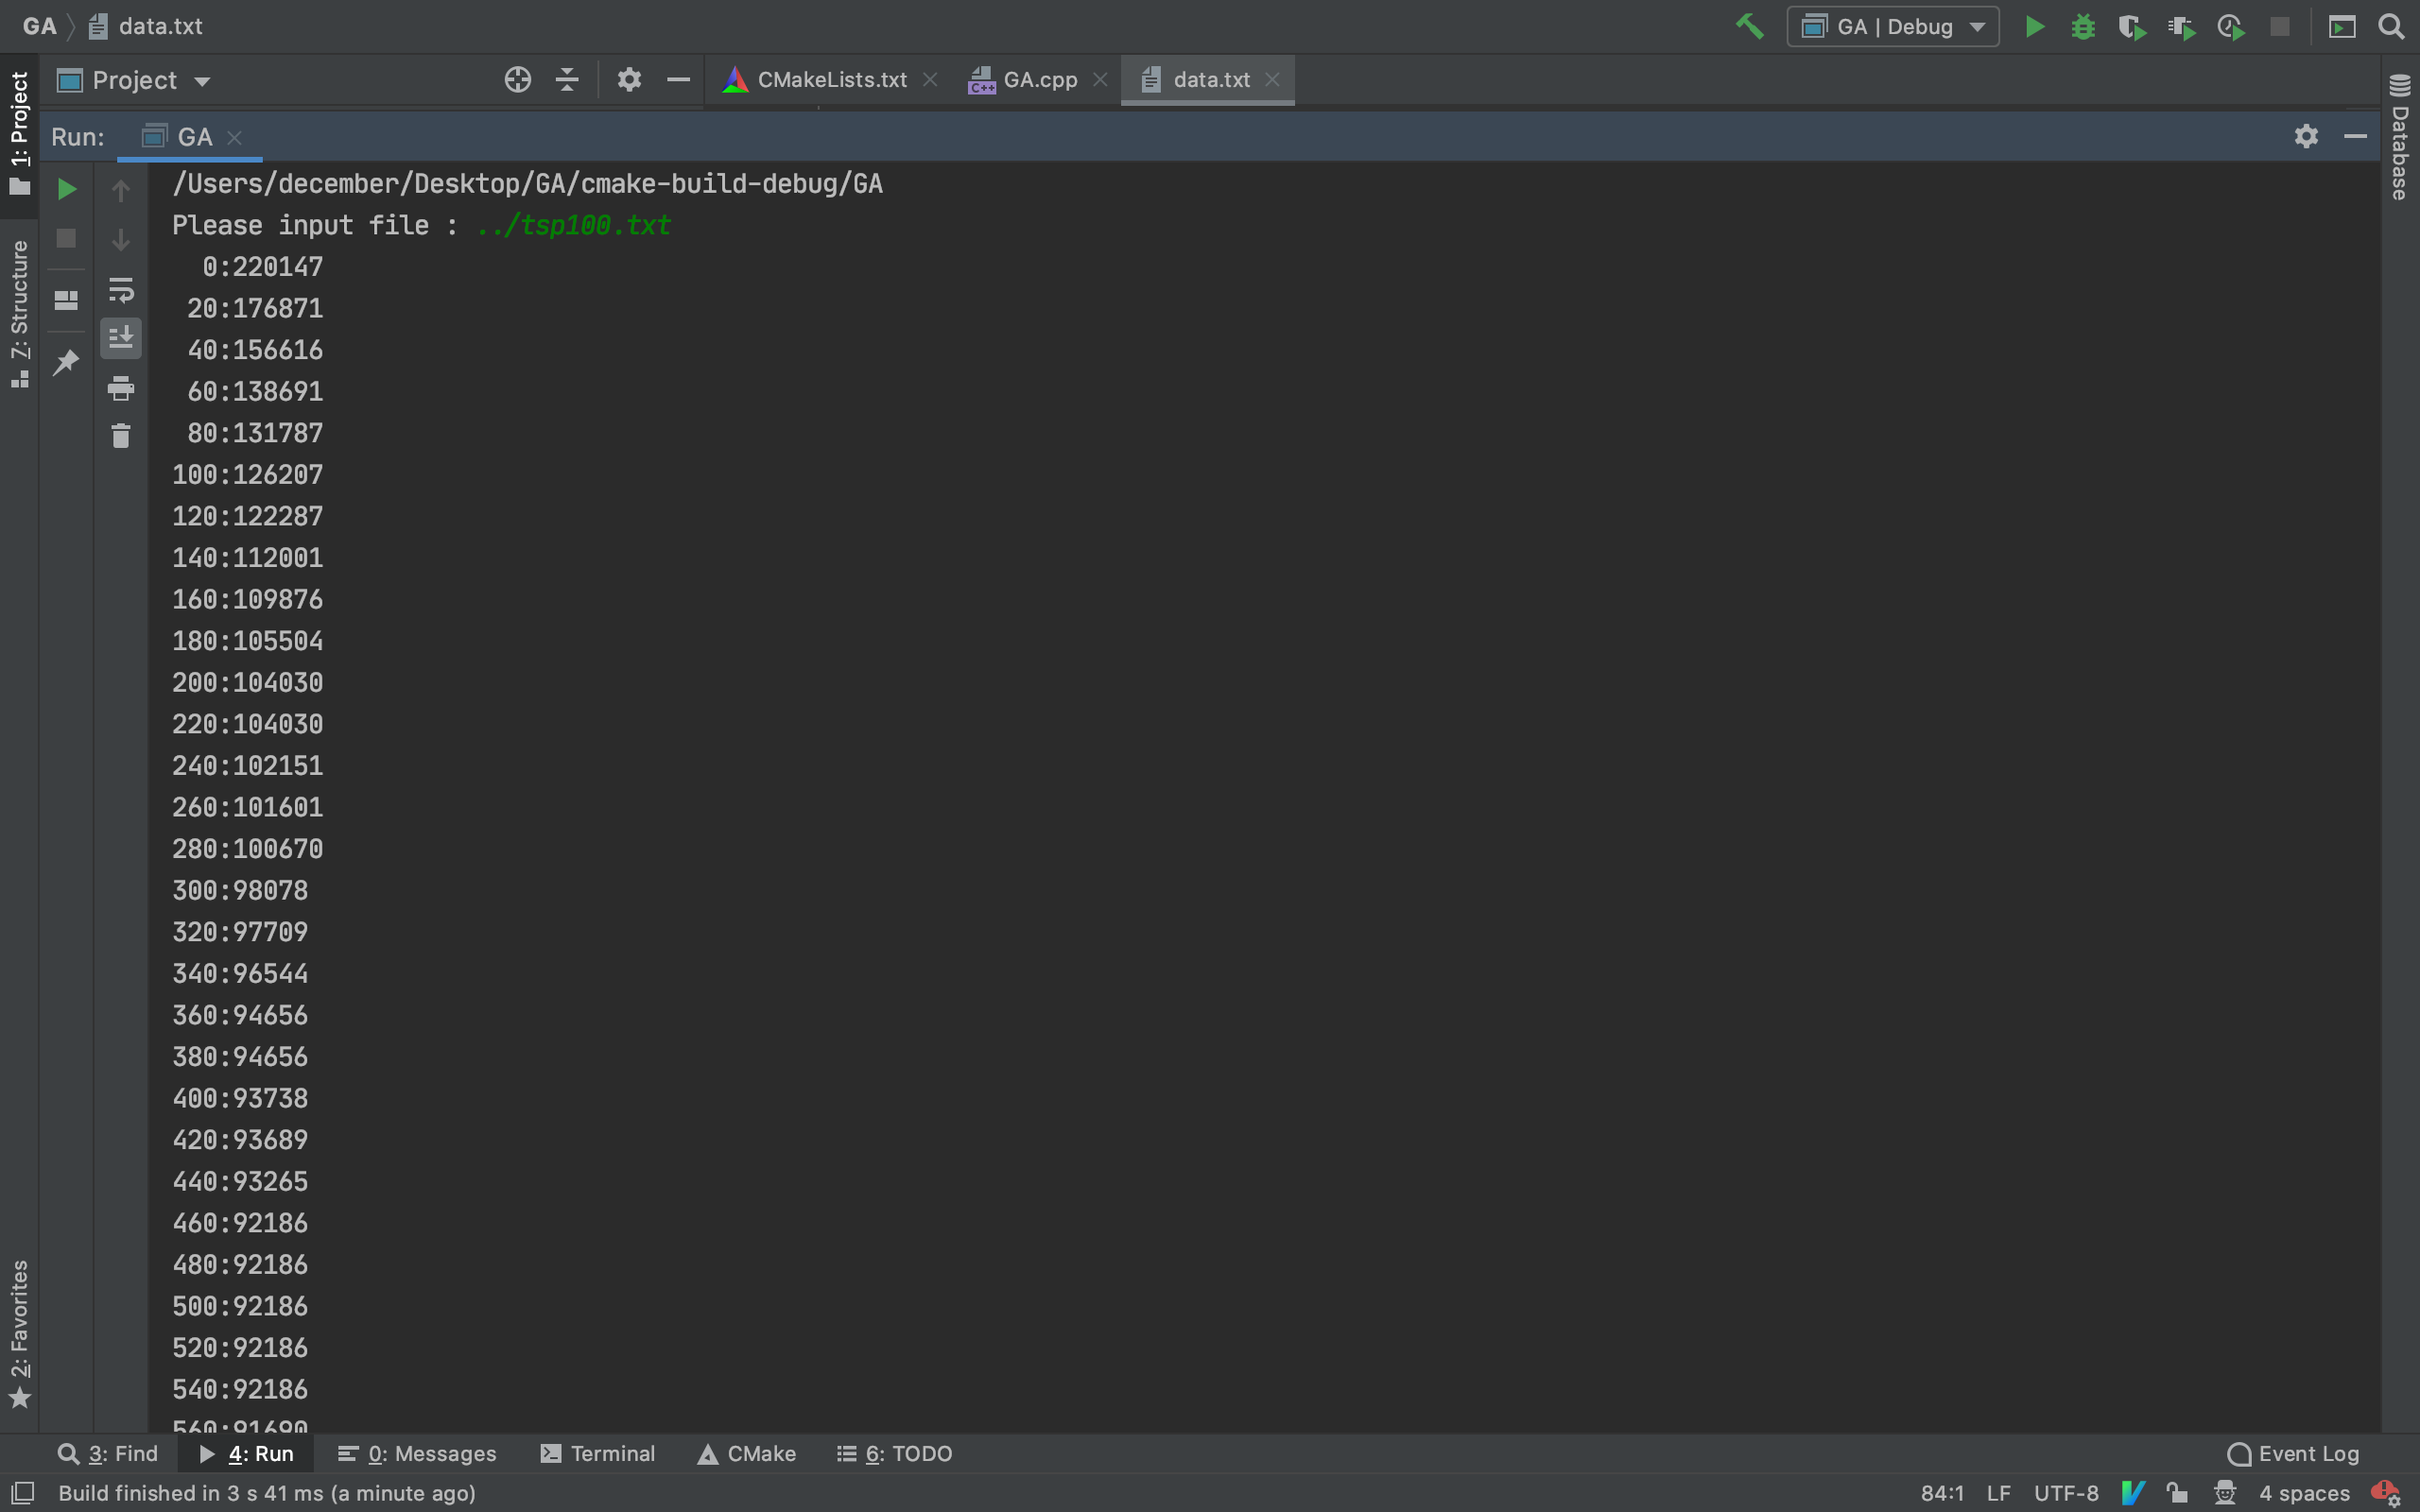
\includegraphics[width=0.45\textwidth]{100}}
    \subfloat{
        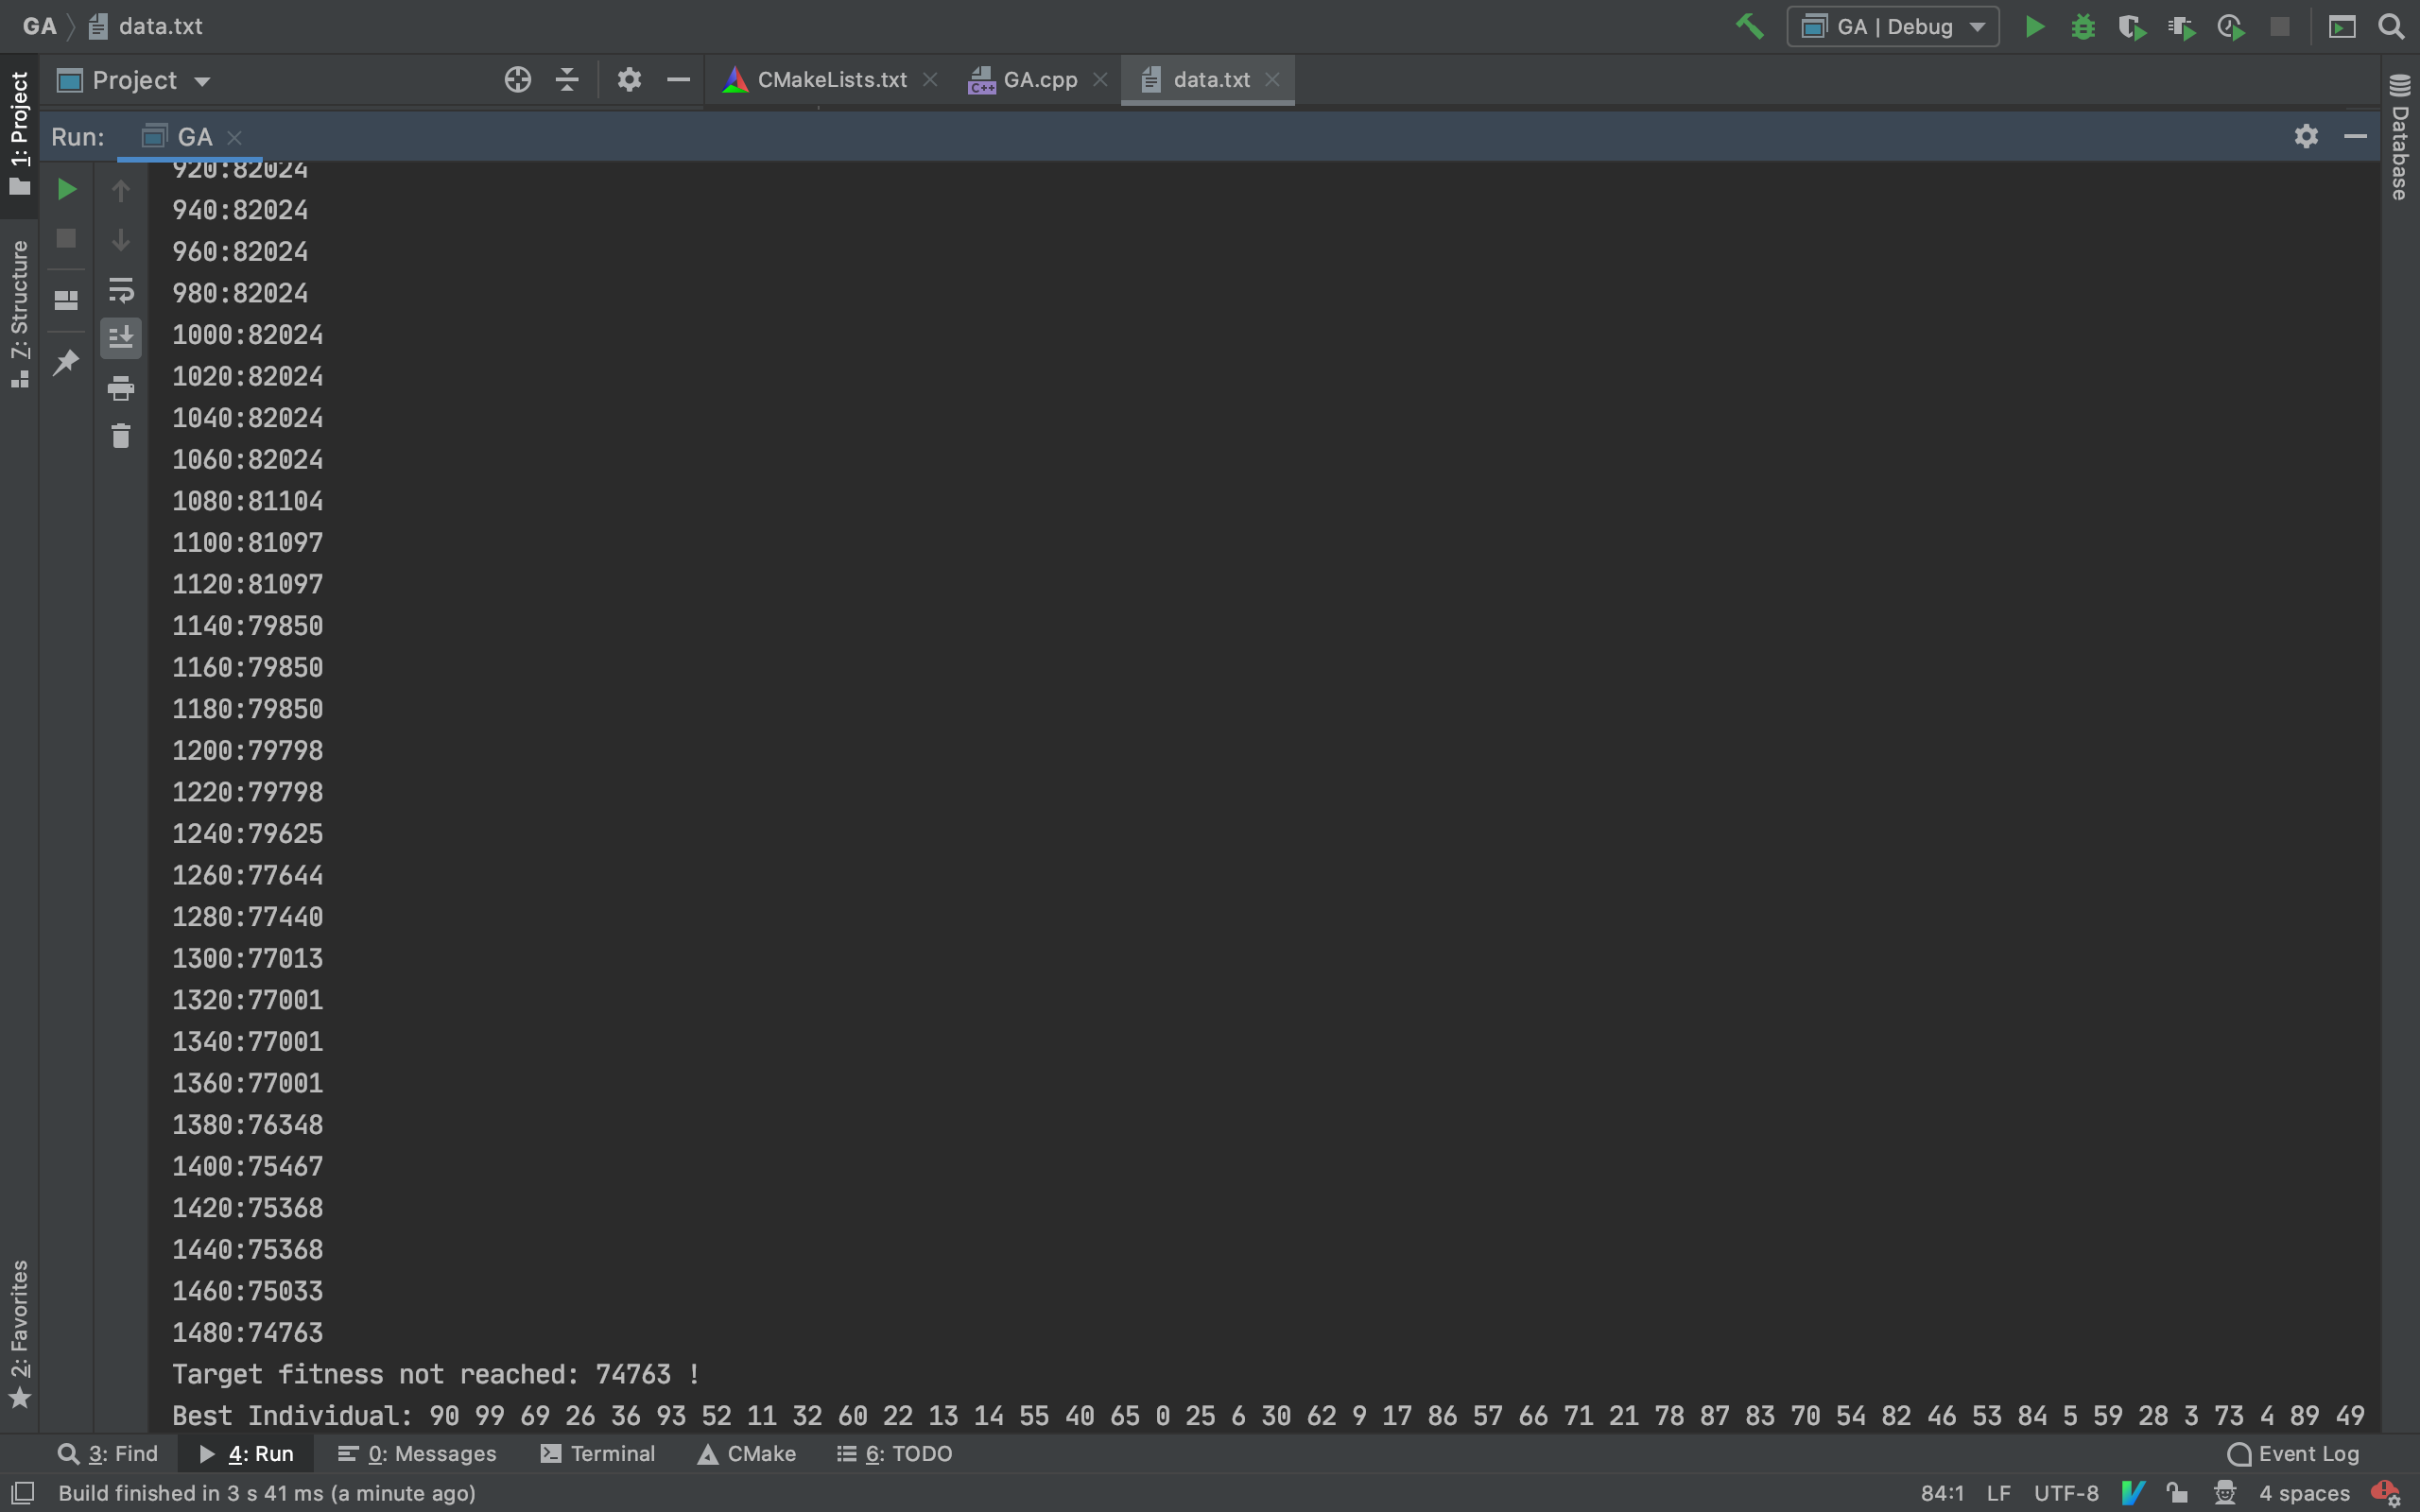
\includegraphics[width=0.45\textwidth]{1002}}
    \caption{tsp100}
\end{figure}

\begin{figure}[H]
    \centering
    \subfloat{
        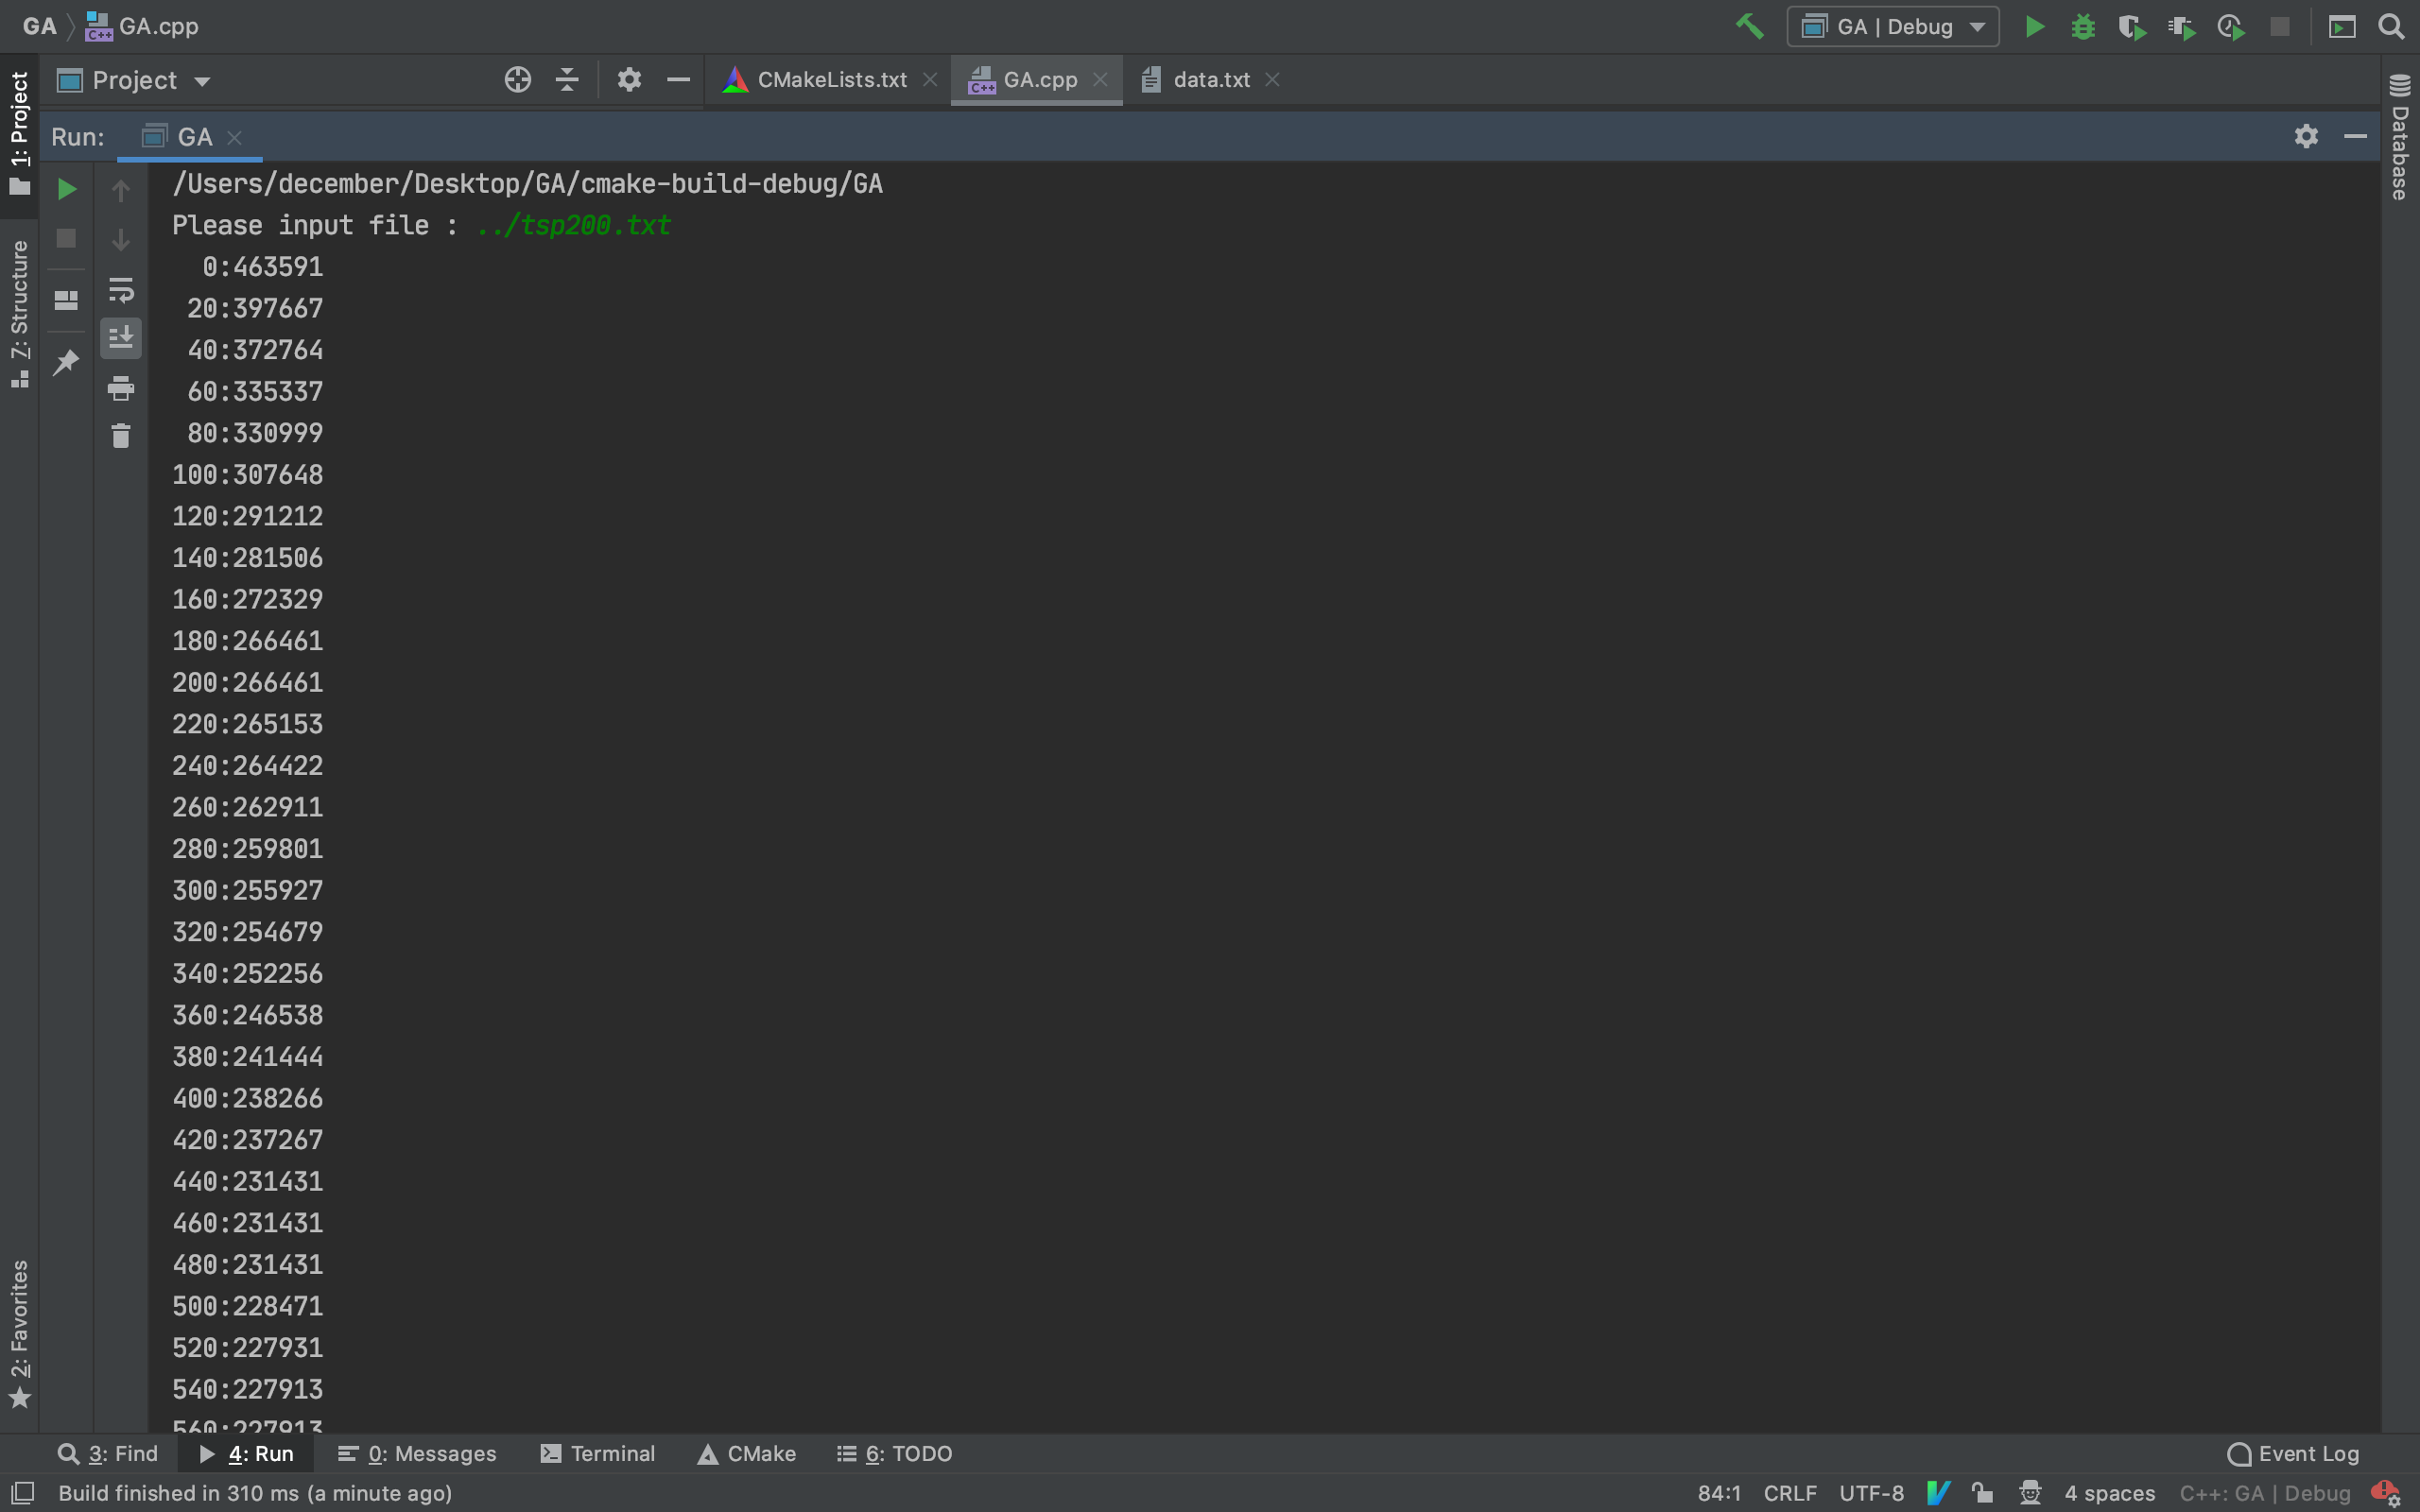
\includegraphics[width=0.45\textwidth]{200}}
    \subfloat{
        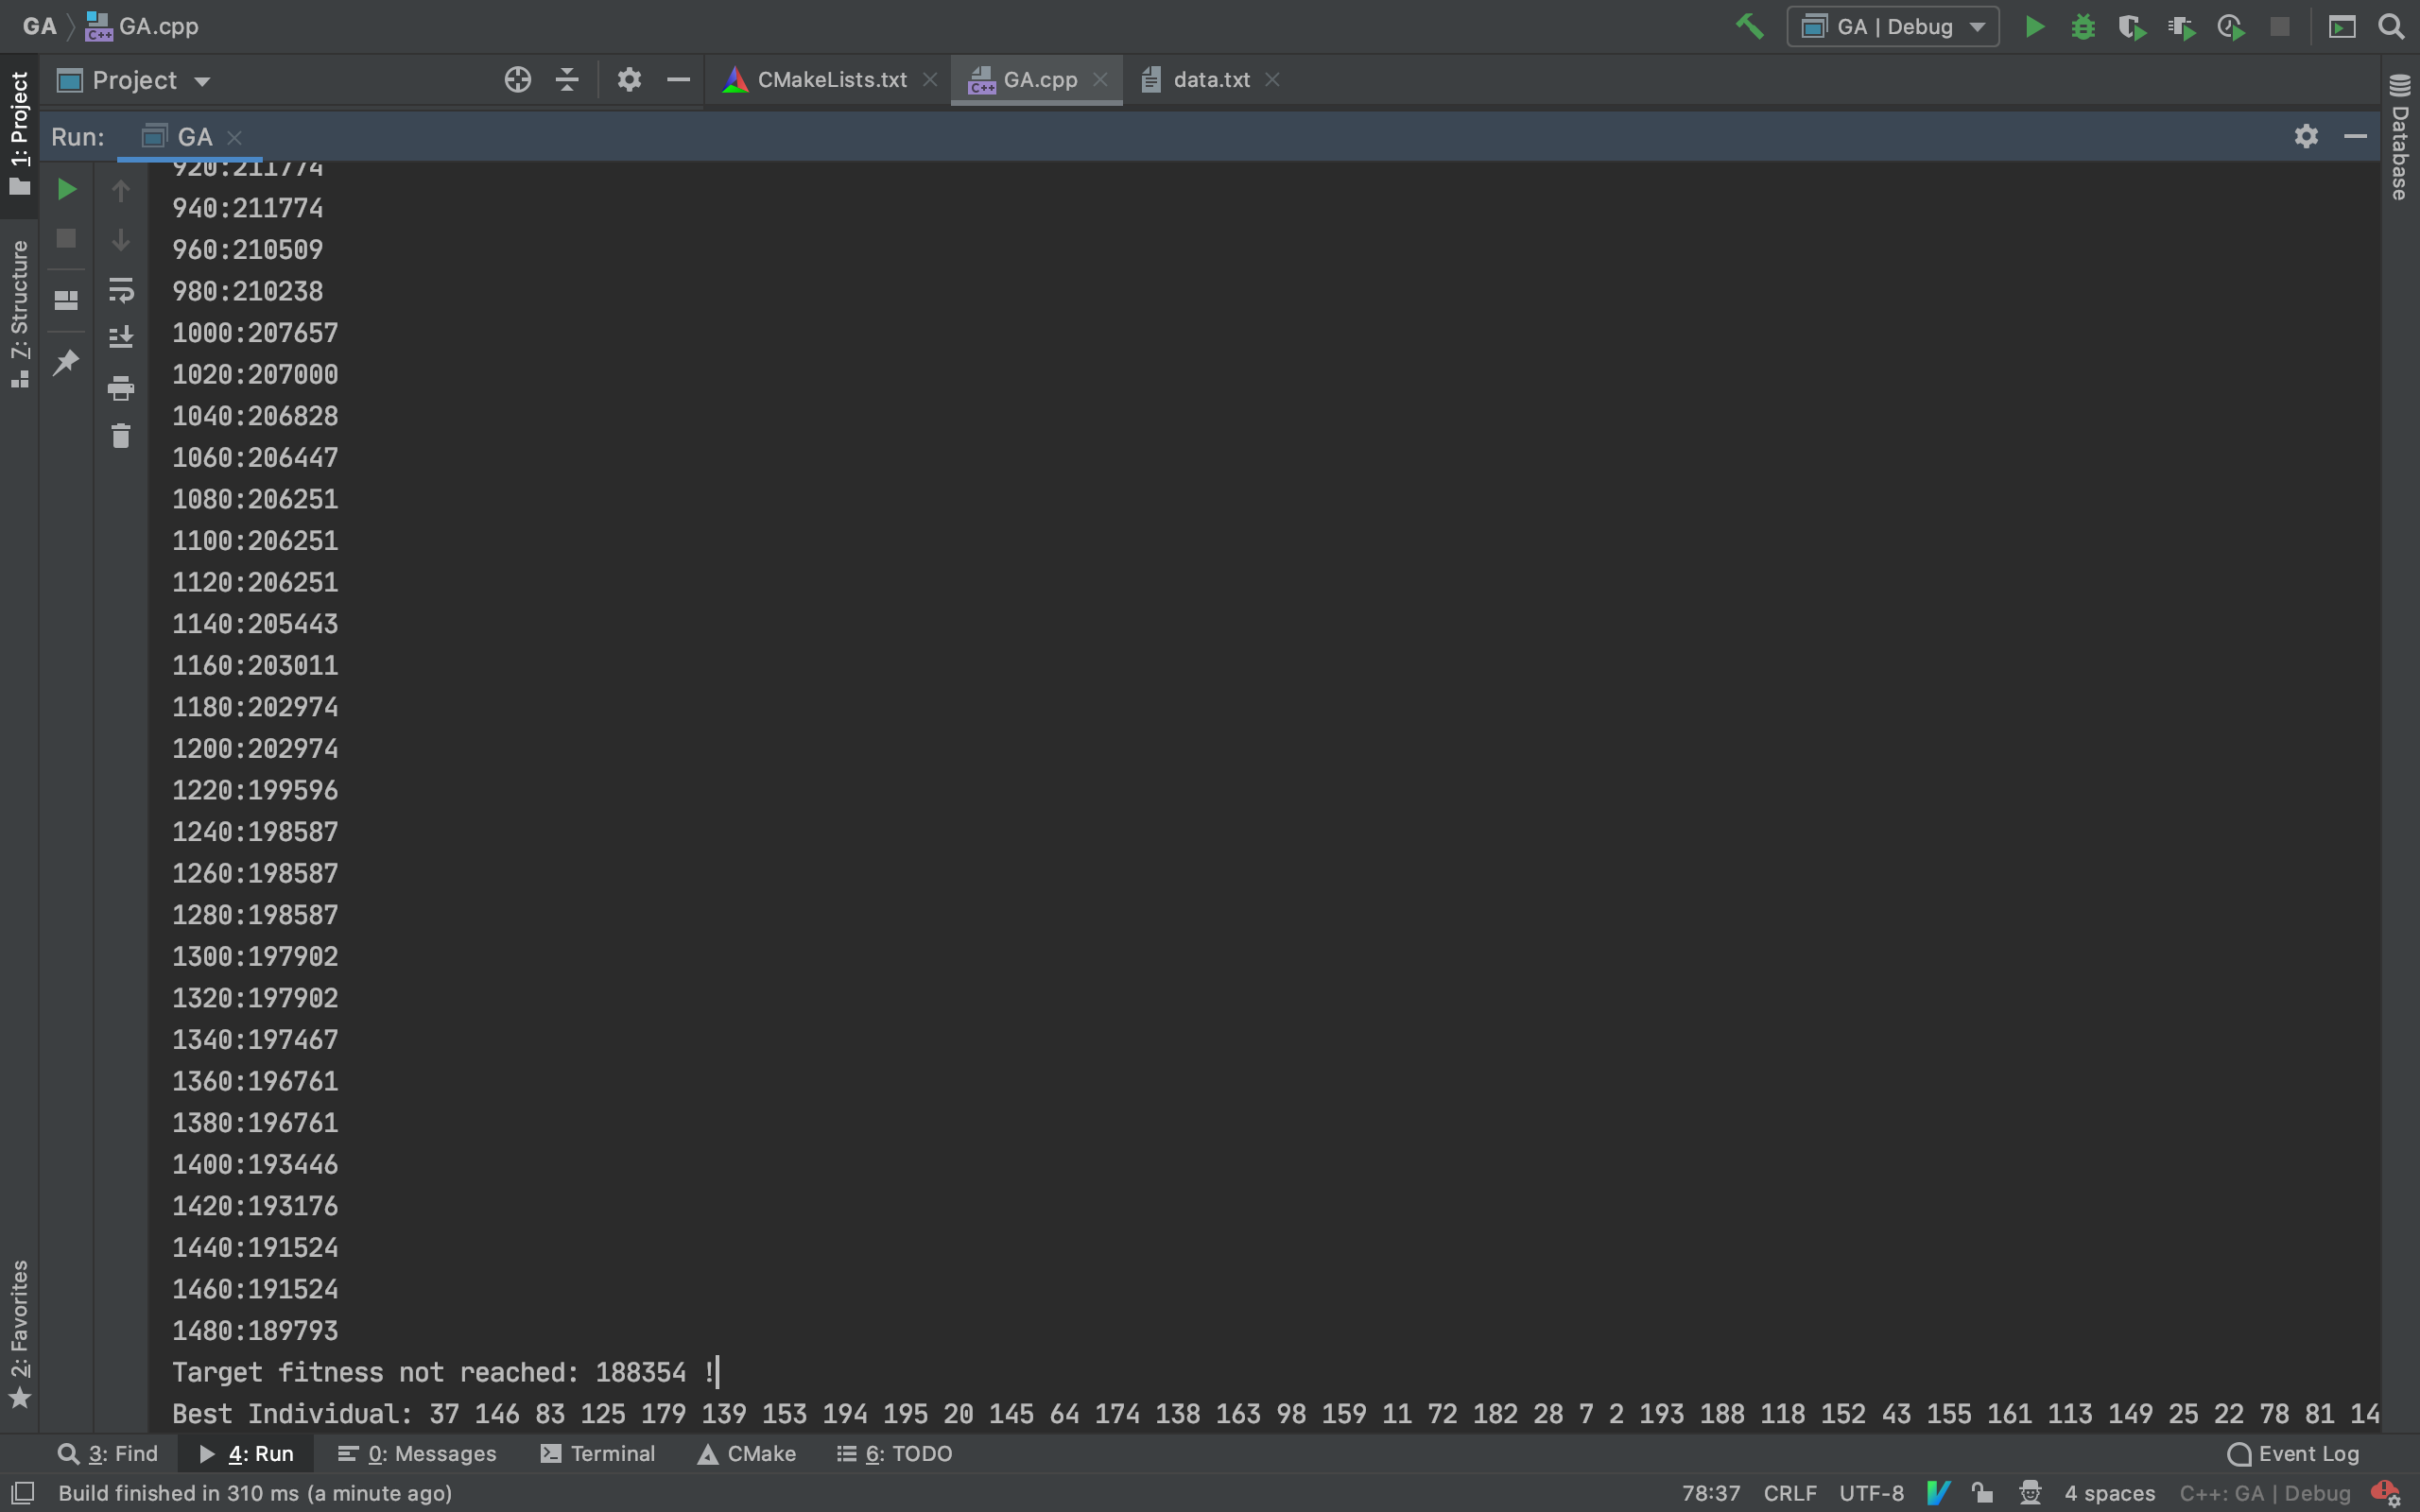
\includegraphics[width=0.45\textwidth]{2002}}
    \caption{tsp200}
\end{figure}

\begin{figure}[H]
    \centering
    \subfloat{
        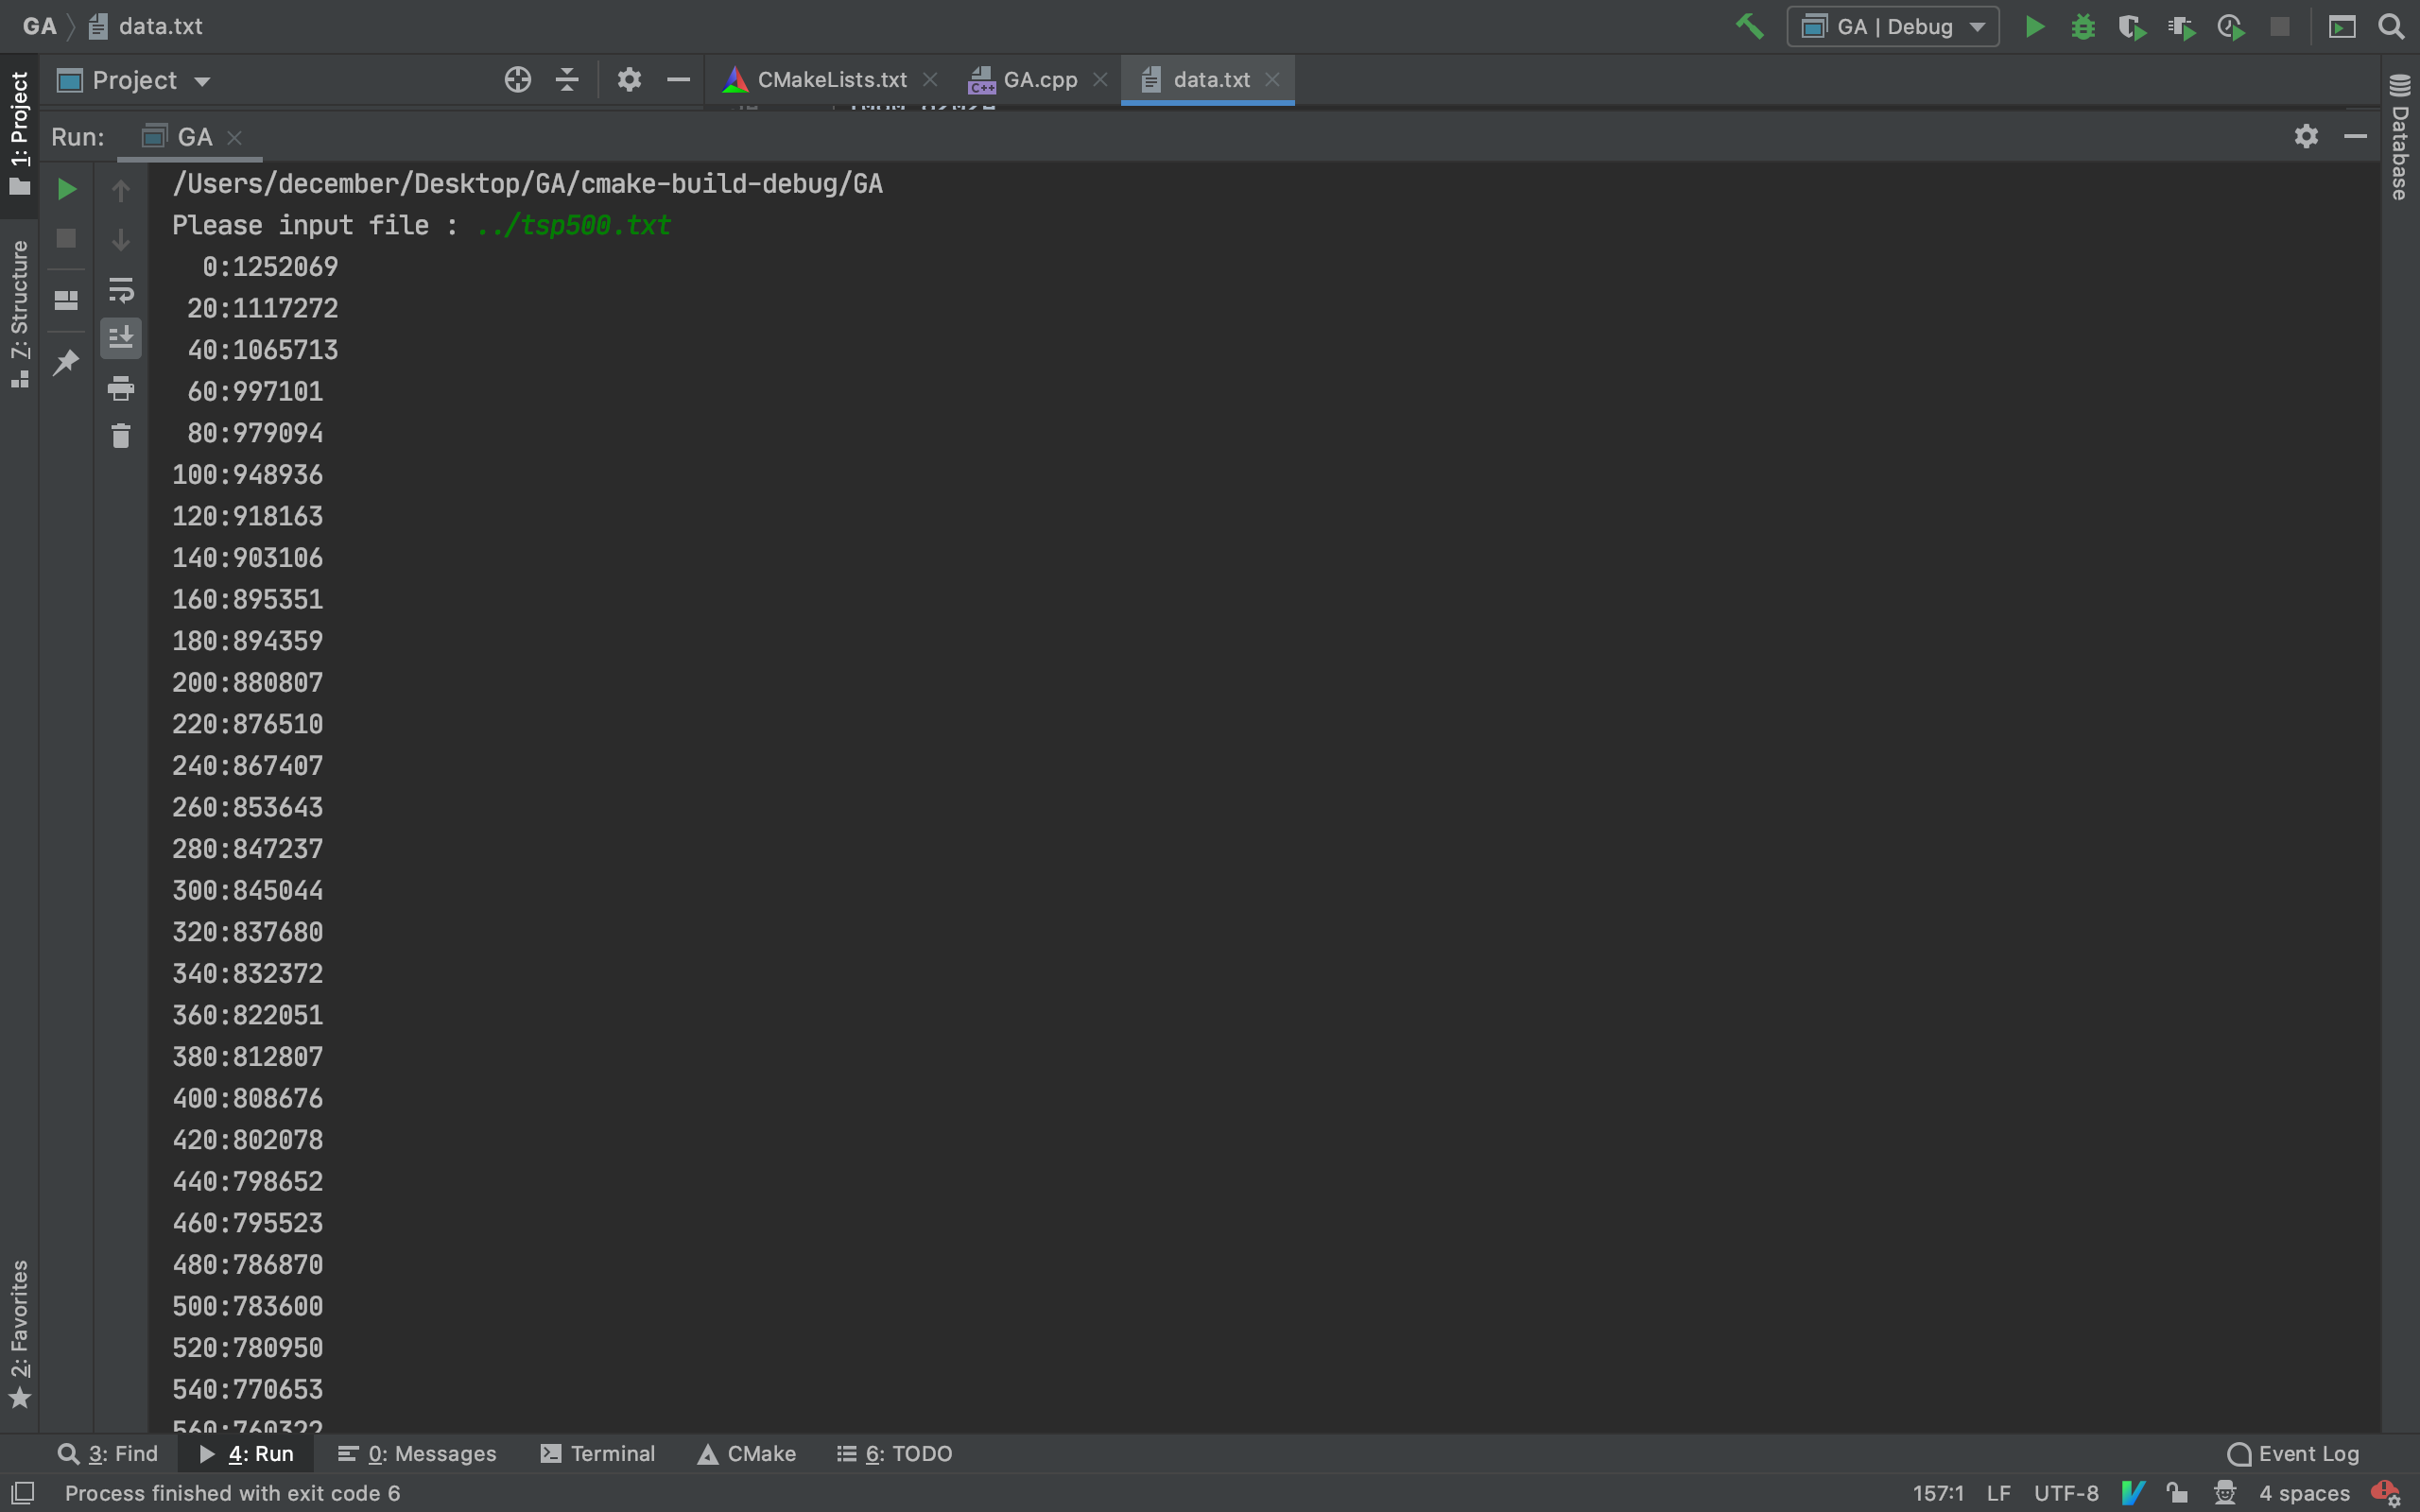
\includegraphics[width=0.45\textwidth]{500}}
    \subfloat{
        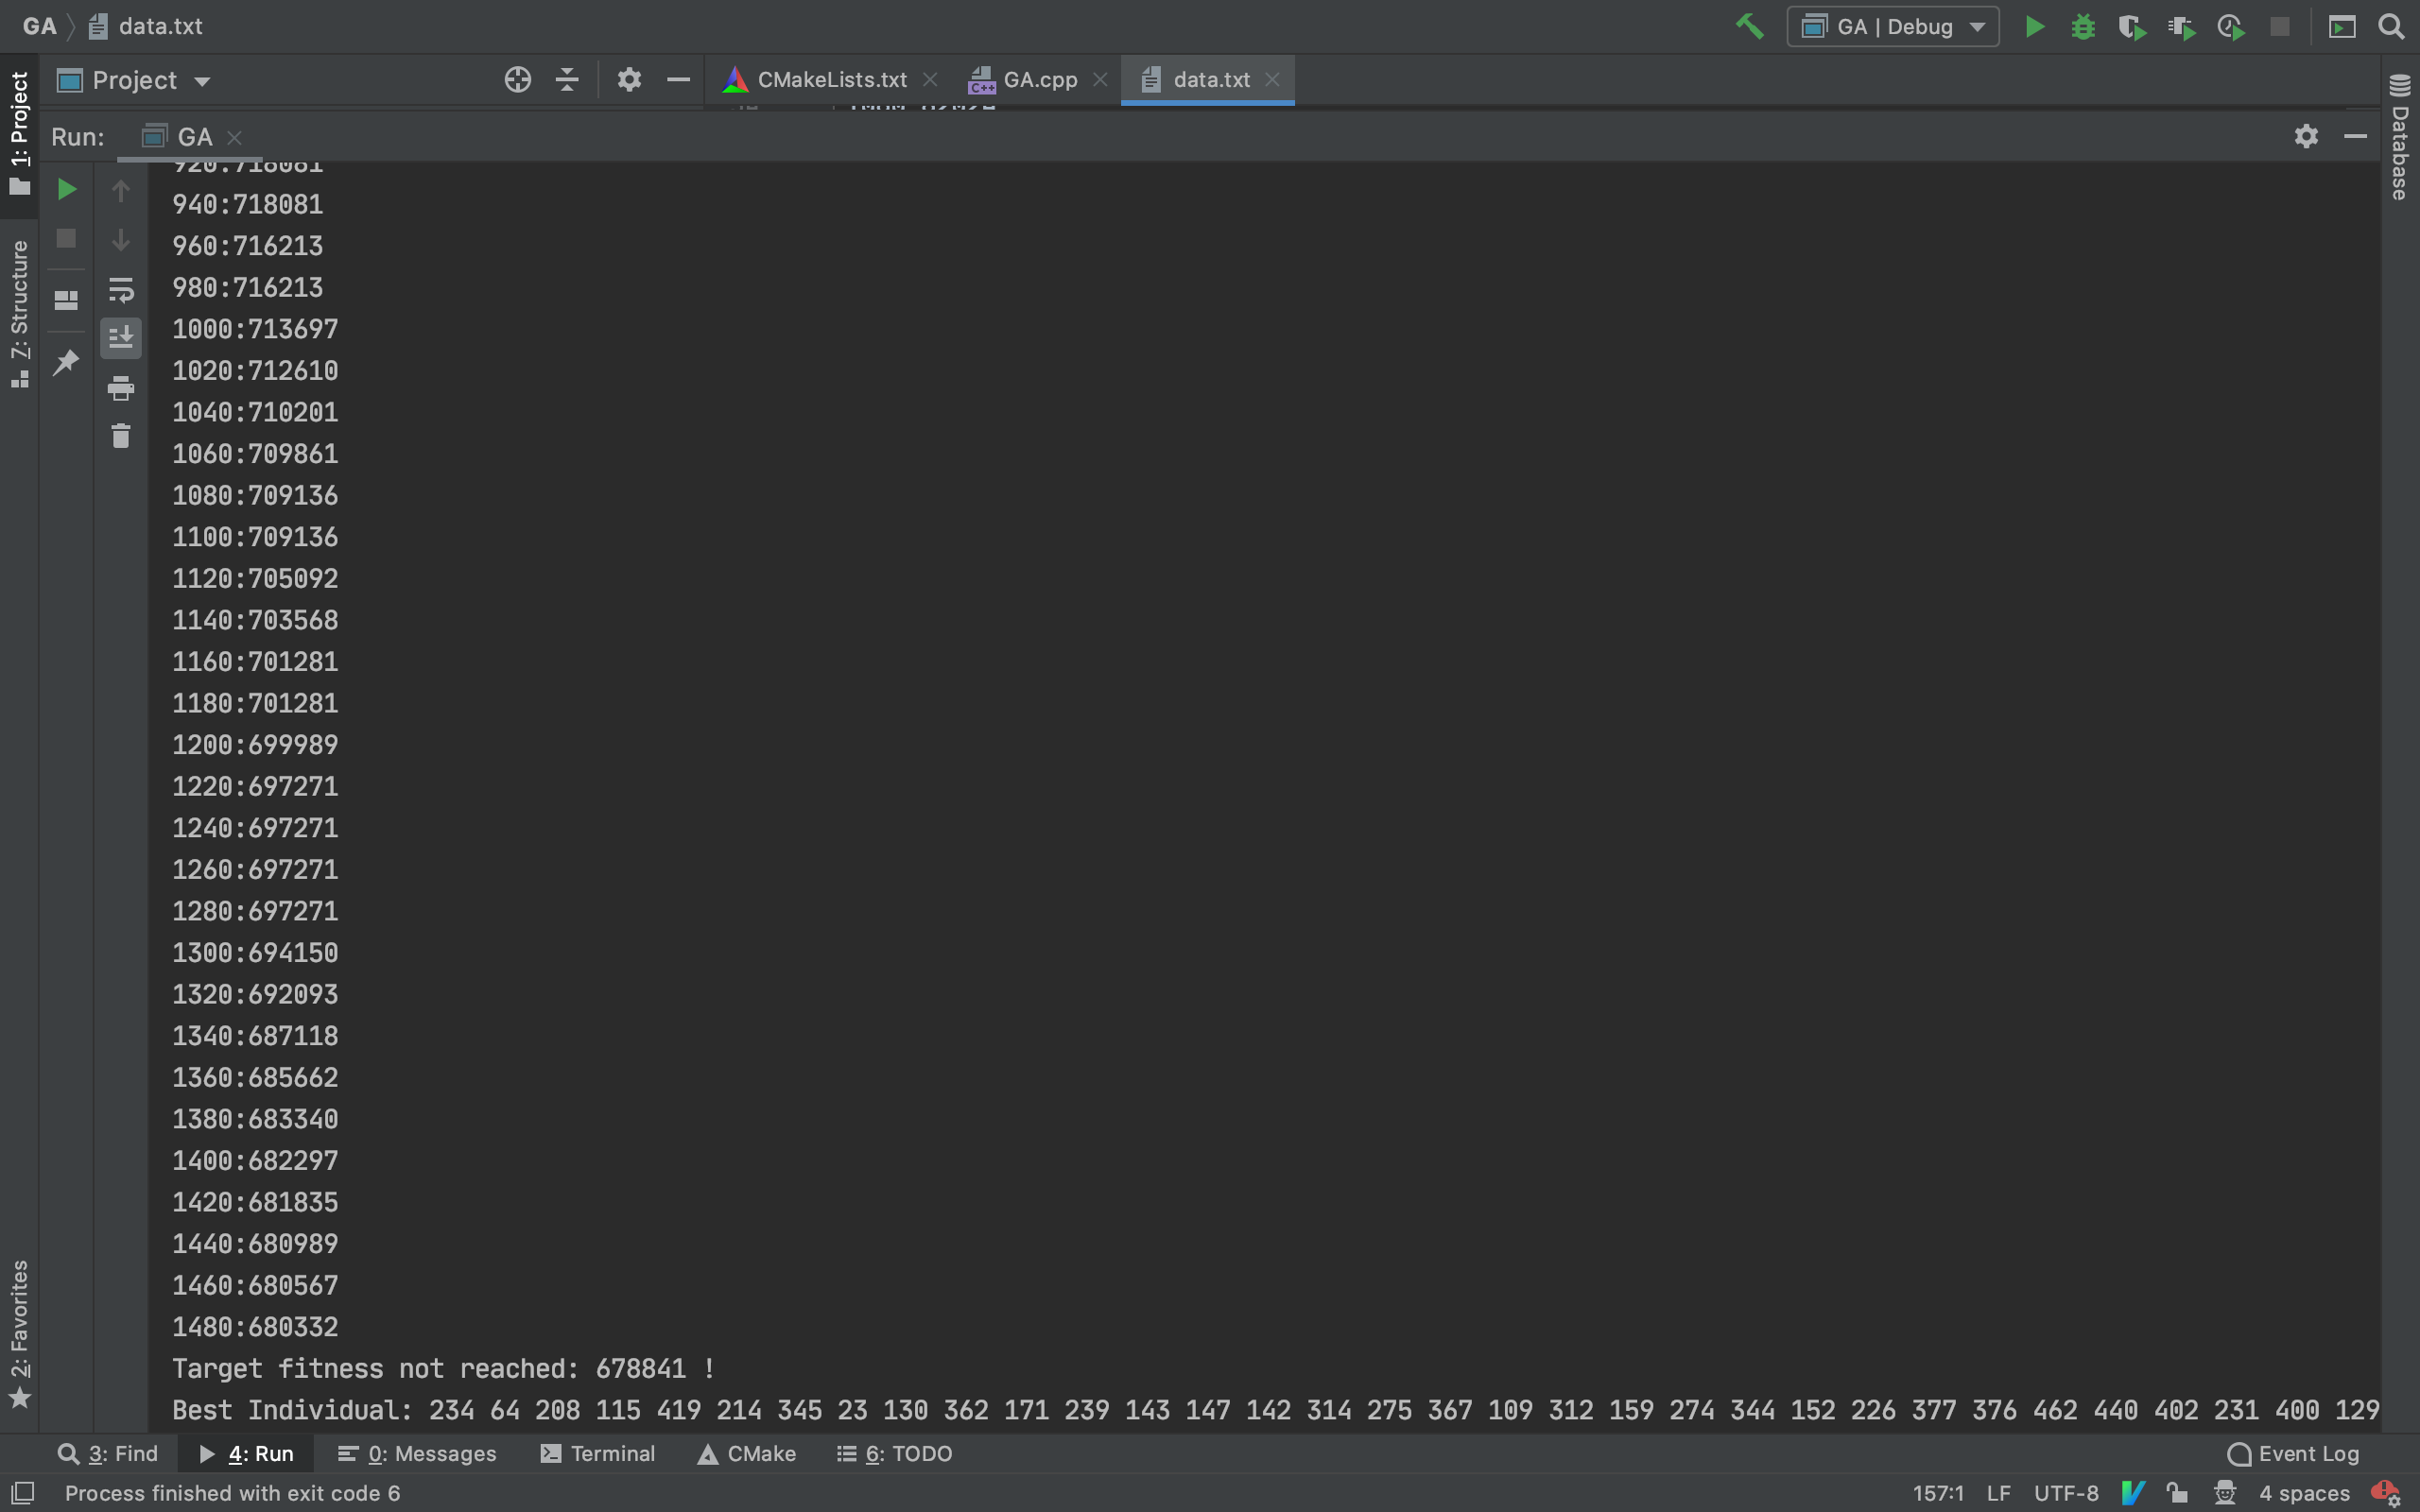
\includegraphics[width=0.45\textwidth]{5002}}
    \caption{tsp500}
\end{figure}

\begin{figure}[H]
    \centering
    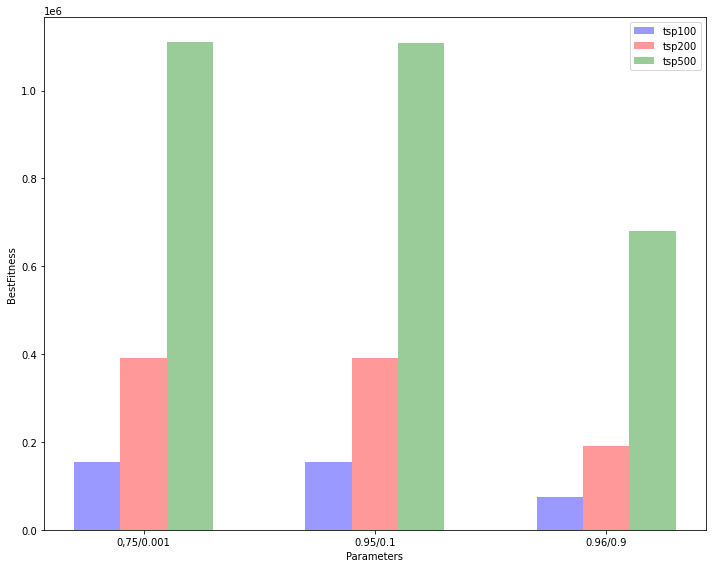
\includegraphics[width=1\textwidth]{compare}
    \caption{Different Parameters}
\end{figure}



\end{document}
